\documentclass[conference, a4paper]{IEEEtran}
\IEEEoverridecommandlockouts
% The preceding line is only needed to identify funding in the first footnote. If that is unneeded, please comment it out.
\usepackage{cite}
\usepackage{amsmath,amssymb,amsfonts}
\usepackage{algorithmic}
\usepackage{graphicx}
\graphicspath{{images/}}
\usepackage{textcomp}
\usepackage{xcolor}
\usepackage{cuted}
\usepackage{capt-of}
\usepackage{hhline}
\usepackage{multirow}
\usepackage{colortbl}
\usepackage{subfigure}
\usepackage{nicematrix}

\def\BibTeX{{\rm B\kern-.05em{\sc i\kern-.025em b}\kern-.08em
    T\kern-.1667em\lower.7ex\hbox{E}\kern-.125emX}}
    
\makeatletter
\newcommand{\linebreakand}{%
  \end{@IEEEauthorhalign}
  \hfill\mbox{}\par
  \mbox{}\hfill\begin{@IEEEauthorhalign}
}
\makeatother
    
\begin{document}

\title{Recognition based indoor positioning at MSK Ghent \\{\large Computervision project group 8, 2021-2022}}

\author{
    \IEEEauthorblockN{Robbe Decorte}
    \IEEEauthorblockA{
        \textit{robbe.decorte@ugent.be}
    }
    \and
    \IEEEauthorblockN{Bram De Bleecker}
    \IEEEauthorblockA{
        \textit{bram.debleecker@ugent.be}
    }
    \linebreakand
    \IEEEauthorblockN{Lance Dewaele}
    \IEEEauthorblockA{
        \textit{lance.dewaele@ugent.be}
    }
    \and
    \IEEEauthorblockN{Benoît D'Haene}
    \IEEEauthorblockA{
        \textit{benoit.dhaene@ugent.be}
    }
    \and
    \IEEEauthorblockN{Lennert Steyaert}
    \IEEEauthorblockA{
        \textit{lennert.steyaert@ugent.be}
    }
}

\maketitle

\begin{abstract}
An indoor positioning program for the MSK Ghent was developed in this article. Videos made by a visitor of the MSK Ghent are used to determine the visitor’s position and the taken path. From those videos, paintings are extracted and compared with a database. The unsupervised painting detection algorithm achieved an F1-score of 85\% and an average intersection of union score of 89\% (for the detected paintings) on a test dataset with 801 samples. To match the extracted paintings with the database one of three different matcher combinations can be used (keypoint-based matching (ORB), feature vector-based matching, or a combination of the previous two). The keypoint-based feature and vector-based matchers were extensively tested and benchmarked to select either an optimal amount of keypoints (in the case of ORB) or the kind of distance metric for the feature vector case. Based on the results we’ve chosen 100 keypoints and as distance metric cityblock and euclidean. The vector generation was executed using the VGG16 deep learning architecture. For the localization, a hidden Markov model was used to predict the changes of the user being in a certain room. Finally, these chances are visualized with colors on a floor plan of the MSK Ghent. The most likely used path is also shown on the floor plan.
\end{abstract}

\begin{IEEEkeywords}
Computer vision, painting detection, unsupervised learning, ORB, hidden Markov model, image similarity, image preprocessing
\end{IEEEkeywords}

\section{Introduction}

Many techniques exist to determine the position of a user or a device relative to its environment. One possible example is visual positioning, which doesn’t rely on communication-based techniques such as satellite navigation or ultra-wideband (UWB) localization. Visual positioning prevents the necessity of a direct line of sight for signal transmissions or the scattering of beacons inside the building, but it does require that the environment contains enough distinctive landmarks unique to its location. Live camera images are compared to a database of previously recorded images that include positional annotations of said landmarks. If the live image matches one of the database images with high certainty, the user is known to be at the location associated with this database image.

 In this paper, we propose a visual positioning solution for indoor localization at the Museum voor Schone Kunsten (MSK) in Ghent (floor plan shown in figure \ref{fig:msk-groundplan}). This proposal helps visitors by providing the current room number, but more importantly the museum curators themselves. It can give insights on frequently used routes in the museum and show which rooms are more popular based on the number of visitors and the average amount of time spent in that room. Each room contains a large number of recognizable landmarks, the paintings themselves (see figure \ref{fig:image-example}). 

Multiple videos of visitors walking around the museum are available. Besides that, we have access to a dataset that contains the paintings belonging to each room and a testing dataset that contains images with positional annotations of the paintings. Section \ref{sec:preprocessing} presents two image preprocessing steps to improve the overall accuracy and performance of the algorithm. The first technique is a way to sample frames based on how blurry the content is. It prevents the frames from entering other stages of the localization pipeline if needed. This section ends with the calibration procedure of the GoPro camera that was used to record parts of the dataset. The unsupervised painting detector is discussed in section \ref{sec:painting-detection} and includes benchmark performance and common causes of failure. Section \ref{sec:painting-matching} explains the matching procedure against the database. All previous components come together in section \ref{sec:localisation}. By combining all parts and extending it with a hidden Markov model, it is possible to accurately determine the location and return the path taken to its current location.

\begin{figure}[htbp]
    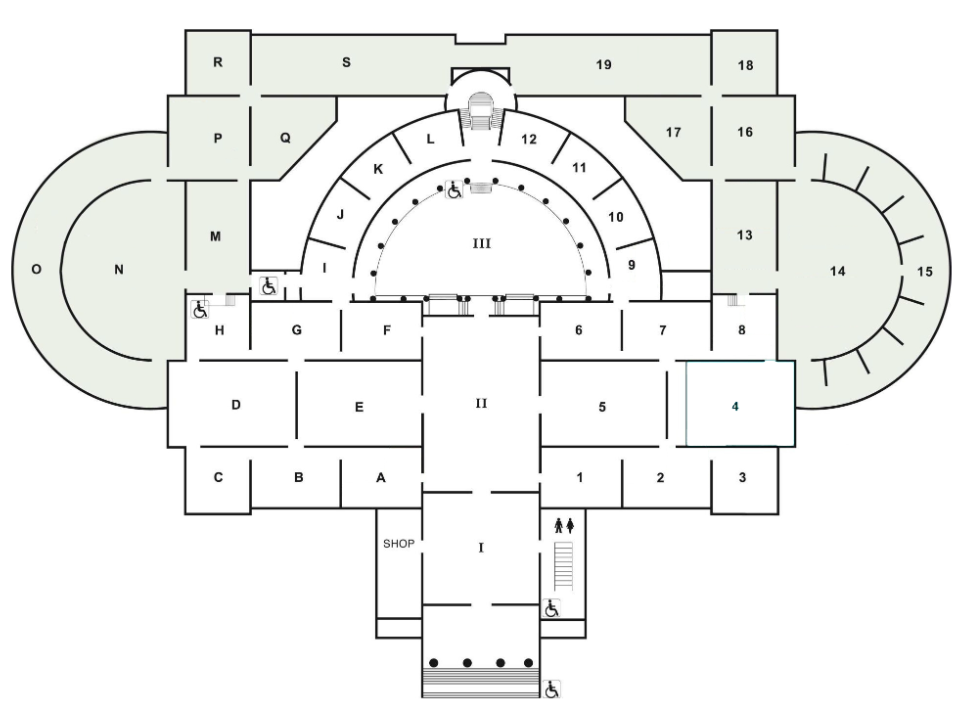
\includegraphics[width=\linewidth]{images/groundplan_msk.PNG}
    \caption{Floor plan of Museum van Schone Kunsten Gent}
    \label{fig:msk-groundplan}
\end{figure}

\begin{figure}[htbp]
    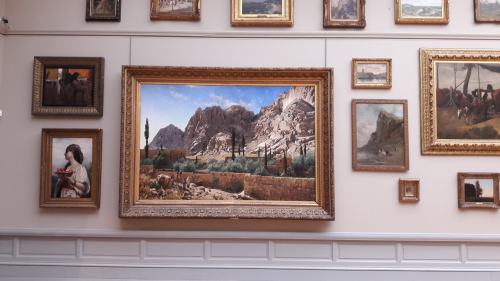
\includegraphics[width=\linewidth]{images/image-example.png}
    \caption{Sample image of the museum}
    \label{fig:image-example}
\end{figure}
\section{Frame processing}
\label{sec:preprocessing}

\subsection{Frame selection using a sharpness metric}
\label{subsec:blur-detection}
% Voor uitleg over accutance
% https://www.cambridgeincolour.com/tutorials/sharpness.htm

Running the detection and matching algorithm on every frame in the video is unfeasible when realtime positioning is required because the time needed to complete every stage takes longer than the available time\footnote{Available time is based on the FPS of the video feed, in perfect circumstances we would match the original FPS with all calculation included.}. If this is ignored, the video stream would be playing in an extreme form of slow motion. Note that it is also possible that some frames may be blurry and thus are a complete waste of computational resources. Motion blur is caused by moving the camera around and  severely hampers the matching of details (edges are less visible, strong keypoints become undetectable, etc.).  The frames will most likely not be matched correctly and should be avoided. Image sharpness is closely related to acutance. It describes how quickly image information transitions at an edge, and so high acutance results in sharp transitions and detail with clearly defined borders \cite{tutorialSharpness}. In practice, only images with high acutance are  wanted  to feed the detection pipeline. That is why a procedure is needed to measure sharpness in an image.

One possible solution to handle this problem is to implement the algorithm proposed by Tong et al. \cite{Hanghang2004}. The proposed scheme makes use of the Haar wavelet transform to decompose a given image into an approximation image and oriented detail coefficients (horizontal, vertical, and diagonal direction). Edges are generally classified based on how sudden the transition is. Immediate transitions can be seen as a Dirac-like structure while slower transitions are more like a skewed step function \cite{Hanghang2004}\cite{712011}. Images normally contain all kinds of edge structures while the images affected by motion blur generally lack strong edges. The general technique to detect a blurry image is to classify and count different kinds of edges on consecutively decomposed images. For each decomposition level, an edge map is created based on the detail coefficients of that level. This results in a pyramid like structure (image dimensions of the approximation reduces every iteration) in which different edge types are counted. The image is classified as blurry if the ratio between Dirac edges and skewed step functions (with a given slope) exceeds a given threshold.

\subsection{Handling camera distortion}

Parts of the videos included in the dataset are filmed with a GoPro camera. This camera contains a so-called fish eye lens. It causes an extreme wide-angle perspective that can be great for an immersive action look but not so much when applying detection techniques to the captured frames. The distortion is especially noticeable for straight lines in the frame. If the line is centered in the frame, it can remain quite straight. But because of the way the lens distortion works, the more the line is moved to the edges of the frame (top, bottom, left, right), the more curved the line will be.

This makes the detection of straight lines more difficult and two versions of the algorithm would be required. One for a \textit{normal} camera and one for cameras with a fish eye lens. Therefore, we need to calibrate the GoPro camera so the distortion effects are reduced. This functionality is implemented in the following OpenCV functions: 

\begin{enumerate}
    \item Point correspondences between multiple frames are found by moving around a rectangular chessboard. The inner corners of the board are automatically detected using \textbf{cv2.findChessboardCorners}. Locations of found corners are refined with the \textbf{cv2.cornerSubPix} (integer to floating-point coordinates). These correspondences act as the input of the calibrateCamera function in the next step.
    \item \textbf{cv2.calibrateCamera} returns the camera matrix, distortion coefficients, rotation and translation vectors (intrinsic and extrinsic camera parameters). This function implements the algorithm proposed by Zhengyou Zhang \cite{Zhang2000}. Results are persisted for each camera type.
    \item \textbf{cv2.undistort} reduces the distortion effects. Note that the resulting image should be cropped using the valid pixel ROI metrics provided by \textbf{cv2.getOptimalNewCameraMatrix}.
\end{enumerate}

%The effectiveness of the procedure above is illustrated using figure \ref{fig:FIXME} (image from the GoPro, before undistort) and figure \ref{fig:FIXME} (after reducing distortion effects). Note that the lines in the second image appear much straighter than before.

% TODO: fotos before en after distortion.
% ga ik skippen denk ik (robbe) geen probleem we begrijpen het gr. Lennert
\section{Painting detection}
\label{sec:painting-detection}

The core of this work is the detection of paintings. For this purpose, an unsupervised segmentation algorithm was designed to extract all visible paintings in any arbitrary image. The essence of the algorithm is to associate straight lines that represent the enclosed region of a painting frame. For convenience, the detector is designed to find rectangular shapes when viewed head-on or quadrilateral shapes when viewed at a different angle.

\subsection{Proposed algorithm}
\label{subsec:proposed-algorithm}

The first step in the detection pipeline is to construct an edge map of a given single-channel image using the Canny operator. Since edge detection algorithms are heavily impacted by noise, the first step should always be to reduce the effects of noise by applying a filter. The original paper by John Canny \cite{Canny1986} suggested using a Wiener filter for optimally estimating the noise component of an image-noise two-component signal. Since this requires knowledge of the noise spectrum it is much easier to apply a Gaussian smoothing filter. All incoming images are resized to a width of 500 pixels and filtered using a 9x9 Gaussian kernel with $\sigma = 1$. The image size is fixed to ensure consistent results throughout the dataset and to speed up the calculations.  Images with higher resolution may cause suboptimal results of the smoothing kernel and would require a variable size of the kernel. The high and low threshold parameters of the Canny operator are calculated using the Otsu method \cite{Fang2009} \cite{greensted}. Its basic principle is to assign every pixel of the image to either foreground or background bucket and to calculate an optimal threshold value based on the intra-class variance. The resulting threshold value minimizes the sum of foreground and background spreads. The resulting edge map of figure \ref{fig:image-example} is shown in figure \ref{fig:edgemap-example}. Note that after applying the Canny operator, some detected edges are disconnected. The results can be improved by dilating the edge map using a 3x3 kernel.

\begin{figure}[htbp]
    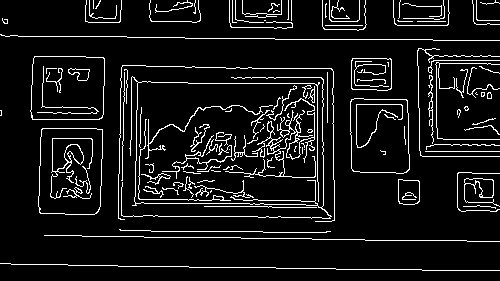
\includegraphics[width=\linewidth]{images/edgemap-example.png}
    \caption{Edgemap of figure \ref{fig:image-example}}
    \label{fig:edgemap-example}
\end{figure}

\textbf{Cv2.findContours} extracts contours using the binary edge map from the previous step. A contour is defined as a curve joining all the continuous points (along the boundary), having the same color or intensity \cite{opencvContours}. Thus the result of this function is a list of groups. Each group consists of points (that are connected to each other) in the binary image. To exclude contours that lie fully within other contours the retrieval mode can be set to \textbf{cv2.RETR\_EXTERNAL}. Contours are sorted by area and limited to the 25 largest to prevent small detected patches that are unusable by the matching algorithm anyway. The next step tries to select contours that are closely related to the shape of a painting frame (squares, rectangles, quadrilaterals, etc.). This implies that we first need to simplify each group of points to a general geometric shape so the corners can be assigned. First of all, the convex hull of the contour is generated and simplified using the \textbf{cv2.approxPolyDP} function to correct small errors in straight lines. Afterward, every contour may be considered a candidate painting if the simplified convex hull can be represented using four points (the corners of the quadrilateral) and its solidity is greater than 60\% (see equation \ref{eq:solidity}). The solidity check prevents the acceptance of contours that are an extreme mismatch compared to their respective convex hull.

\begin{equation}
    \label{eq:solidity}
    Solidity = \frac{Contour \; Area}{Convex \; Hull \; Area}
\end{equation}

The final step in the algorithm is to rectify every contour that satisfies the previous criteria. This is easily done as the corners of the quadrilaterals are known. The matching algorithm and subsequent steps require the inputs to be rectangular to ensure optimal results.

The rectified image crops are passed through the blur detection scheme from section \ref{subsec:blur-detection}. Blurry or vague crops are far more likely to cause a miss classification in the matcher. This mainly occurs when paintings are detected with an acute viewing angle.

\begin{figure}[htbp]
    \subfigure[All contours found on figure \ref{fig:image-example}]
    {
        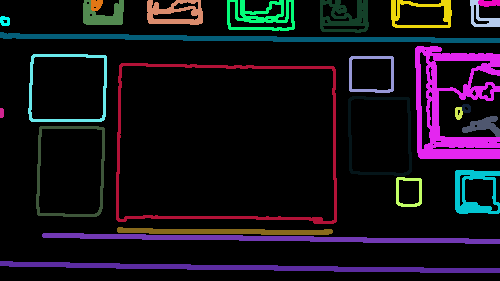
\includegraphics[width=.9\linewidth]{images/contours_all_example.png}
        \label{fig:contours_all}
    }
    \subfigure[Filtered contours, amount of corners and solidity checks applied]
    {
        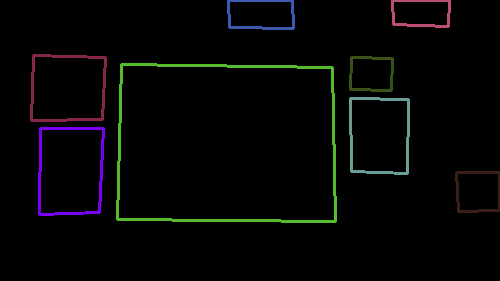
\includegraphics[width=.9\linewidth]{images/contours_filtered_example.png}
        \label{fig:contours_filtered}
    }
    \subfigure[Contours drawn on the original image]
    {
        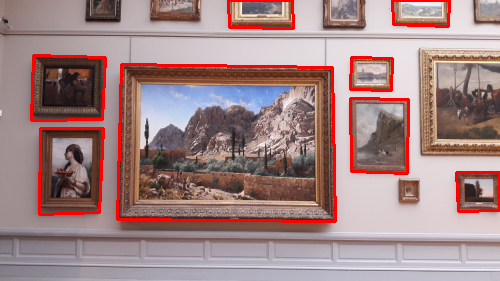
\includegraphics[width=.9\linewidth]{images/contours_filtered_image_example.png}
        \label{fig:contours_on_image}
    }
    \caption{Visualization of the contour filtering procedure (every color represents a different contour)}
    \label{fig:contours}
\end{figure}

\clearpage
\begin{strip}
    \centering
    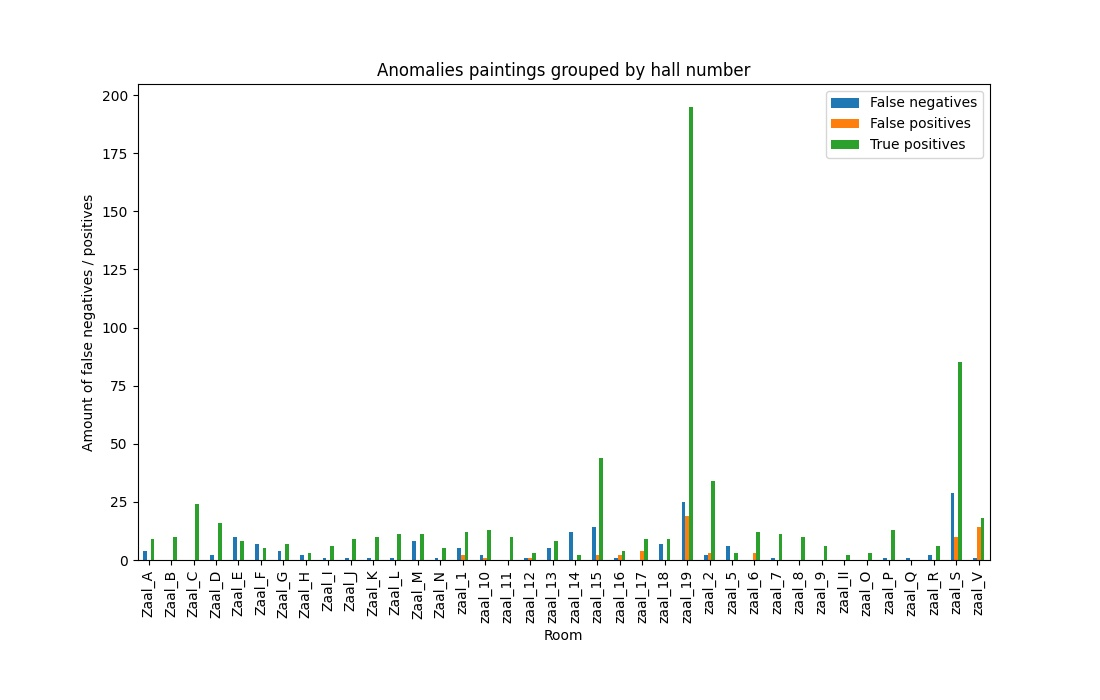
\includegraphics[width=\linewidth]{images/grouped_by_hall_include_TP.jpg}
    \captionof{figure}{Benchmark results displaying a histogram of true positives, true negatives and false negatives}
    \label{fig:benchmark-all}
\end{strip}

\begin{strip}
    \centering
    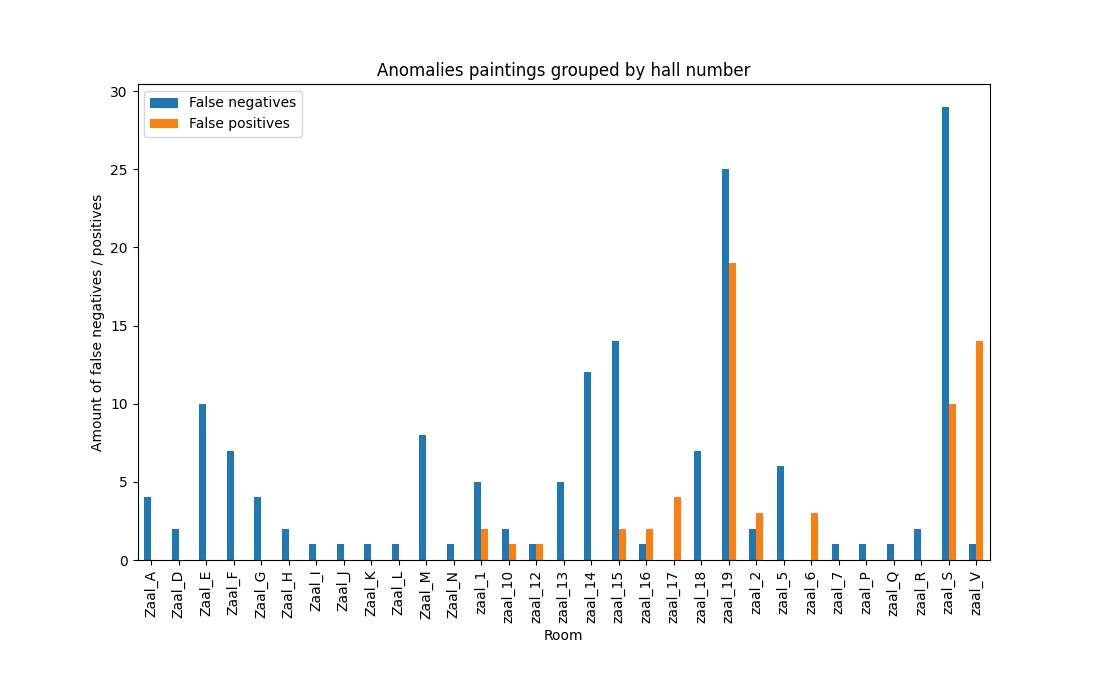
\includegraphics[width=\linewidth]{images/grouped_by_hall.jpg}
    \captionof{figure}{Benchmark results with true Positives omitted}
    \label{fig:benchmark-notp}
   
\end{strip}

\subsection{Benchmark results}

The quality of the painting detector was assessed using a validation dataset and a CSV file that contains the corners of all paintings in the images in the validation set. The results are shown as a confusion matrix in table \ref{tab:confusion_matrix_benchmark} and correspond to a $recall = 0.8065$, $precision = 0.9137$ and  $F1 = 0.8568$. For the detected paintings (646 detected paintings for 801 paintings in the dataset), we achieved an average intersection over union score (IOU) of $0.8934$. The distribution of IOU scores is displayed in figure \ref{fig:IOU-distribution} and is further elaborated on in section \ref{subsec:detection-failure}.

\begin{table}[htbp]
    \caption{Confusion matrix of the benchmark dataset}
    \begin{center}
        \begin{tabular}{l|l|c|c|c}
            \multicolumn{2}{c}{}&\multicolumn{2}{c}{Ground truth}&\\
            \cline{3-4}
            \multicolumn{2}{c|}{}&Positive&Negative&\multicolumn{1}{c}{Total}\\
            \cline{2-4}
            \multirow{2}{*}{Predicted}& Positive & $646$ & $61$ & $707$\\
            \cline{2-4}
            & Negative & $155$ &  & \\
            \cline{2-4}
            \multicolumn{1}{c}{} & \multicolumn{1}{c}{Total} & \multicolumn{1}{c}{$801$} & \multicolumn{    1}{c}{} & \multicolumn{1}{c}{$801$}\\
        \end{tabular}
    \end{center}
    \label{tab:confusion_matrix_benchmark}
\end{table}


\begin{figure}[htbp]
    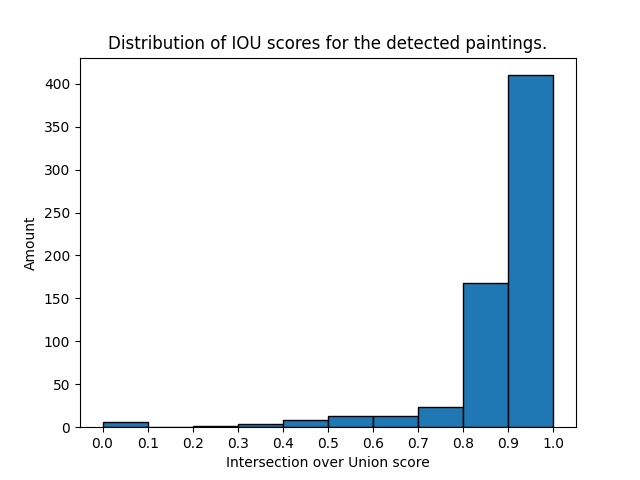
\includegraphics[width=\linewidth]{images/IOU_distribution.jpg}
    \caption{Intersection over union distribution of the detected paintings in the benchmark set}
    \label{fig:IOU-distribution}
\end{figure}



\subsection{Common causes of failure}
\label{subsec:detection-failure}

Figure \ref{fig:common-error-noframe} shows one of the most common detection errors, the exclusion of the painting frame. These are detections that correspond with an IOU score between $0.75$ and $0.95$ (see figure \ref{fig:IOU-distribution}). This doesn't pose too much of a problem since the actual painting information is preserved. However, all the frame information which may contain strong keypoints to match is lost. Those keypoints may be included in the database representation of the ground truth images.

Other common circumstances when a painting is not or less accurately detected are:

\begin{enumerate}
    \item Painting frame is not completely visible in the image.
    \item The difference between the painting background and the wall is not strong enough to be detected as a line.
    \item Shadows caused by the painting frame commonly form a strong edge and are included in the painting contour. This causes a lower IOU score for the detection.
    \item Next to most of the paintings hangs a small plaque (containing information) that is falsely classified as a painting when its color is different from the wall color.
    \item Hall 14 is plastered with a wallpaper that contains quadrilateral shapes which interfere with the contours of the paintings and causes a very large amount of false negatives. This behavior can be verified using figure \ref{fig:benchmark-notp}.
\end{enumerate}

\begin{figure}[htbp]
    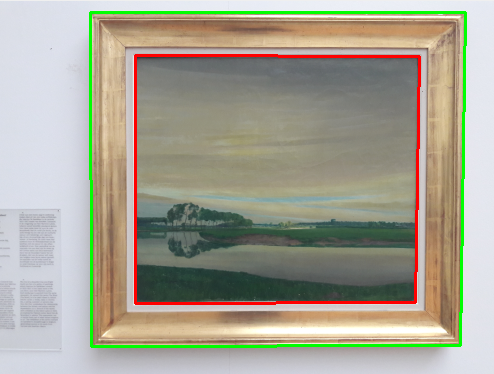
\includegraphics[width=\linewidth]{images/common-error-noframe.png}
    \caption{One of the most common errors (the picture frame is not included in the detection), green shows the ground truth bounding box and red is the predicted one}
    \label{fig:common-error-noframe}
\end{figure}
\section{Painting matching}
\label{sec:painting-matching}

The elaboration of the painting matching consists of two approaches which are discussed in \ref{subsec:Keypoint matching} and \ref{subsec:Feature vector matching}. 

Realtime painting matching must have preprocessing, meaning extraction of keypoints, features and storing it into a database beforehand. The project code contains code to generate such a database. This database will be used to compare a particular painting frame with all it's contents.

\subsection{Keypoint matching}
\label{subsec:Keypoint matching}
The keypoint matching approach relies on Oriented Fast and Rotated BRIEF (ORB) feature detection. ORB is an alternative to SIFT and SURF. These algorithms are patented while ORB is not. \cite{opencvOrb}

According to reference \cite{orb_original_paper} ORB is faster than SIFT or SURF. However, in general ORB has lower correct matching results than SIFT or SURF. \cite{orb_surf_sift_evaluation} Considering the application, time is the more important factor.

Practically, two drawbacks have to be taken into account when using ORB. At first, ORB is not scale-invariant. Thus the detected images should be scaled back to the original size of the image painting stored in the database. For this application, all images are scaled with a fixed width of 800. The second drawback is the influence due to shearing. Matching sheared images implies lower matching scores. \cite{orb_surf_sift_evaluation} This particular drawback is countered by the rectification step.

Another practical issue due to blurry painting detection was established. Blurry images can cause lots of wrong matching results. This issue is mainly prevented by the wavelet filters as described in \ref{subsec:blur-detection}.

In addition to the choice for ORB, the correct matching algorithm had to be determined. OpenCV provides two types of matching algorithms: Fast Library for Approximate Nearest Neighbors (FLANN)-based and brute-force (BF)-based. FLANN matching works faster than BF matcher in case of a large dataset (high amount of key points). Considering the acceptable results (discussed below) based on BF matching the FLANN version wasn't used. \cite{opencv_matching}


%https://docs.opencv.org/4.x/d3/da1/classcv_1_1BFMatcher.html


%https://ieeexplore.ieee.org/abstract/document/6126544?casa_token=CE2fQN6_JwIAAAAA:Inx7X3B3EFlZwekm56UJ4MjTaydpL0emtOb9sEuQmkPS037HKoHzsNvr_KFYqMiwOKrJCe3HgJA

%https://www.inderscienceonline.com/doi/abs/10.1504/IJFE.2021.118910

ORB relies on one important variable, the number of key points (features called in OpenCV). Changing this variable should result in a difference in the matching score, distances between matches, and execution time.

Table \ref{tab:keypoint_feature_variation} shows us the positive and negative matches for each amount of keypoints. In total 437 images were evaluated, they were retrieved from the given dataset. As can be seen in table \ref{tab:keypoint_feature_variation} only a slightly better score is reached when increasing the number of keypoints above 100.  Based on this result the final solution is restricted to 100 keypoints. Only the 20 largest distances (keypoint distance) for a particular image are summed to obtain a distance value for each image in the database.
%true/false matching


\renewcommand{\arraystretch}{1.2}
\begin{table}[htbp]
    \caption{Keypoint/feature variation correctness results}
    \centering
    \begin{center}
        \begin{tabular}{ |c|c|c|c|  }
        %  \hline
        %  \multicolumn{4}{|c|}{Keypoint/feature variation correctness results.} \\
         \hline
         No. keypoints& Positive matches &Negative matches&Mean score (\%)\\
         \hline \hline
         50  & 402 & 35 & 91.99\\
         \hline
         100 & 423 & 14 & 96.80\\
         \hline
         200 & 424 & 13 & 97.03\\
         \hline
         300 & 425 & 12 & 97.24\\
         \hline
        \end{tabular}
    \end{center}
    \label{tab:keypoint_feature_variation}
\end{table}

Distance distributions for matches are also interesting to determine useful information about the matching. Figure \ref{fig:bxplt_distances_keypoints} shows the distance distribution for the correct and incorrect matches. The correct distance matching distribution shows many outliers in the case of the matcher with only 50 keypoints. The amount of outliers decreases as the number of keypoints/features increases. The median for each scenario also decreases as the amount of features increases. It implies fewer high matching distances. The same findings are reflected in the case of incorrect matches. In addition, it can be determined that the distance range for the correct and incorrect matches shrinks as the number of keypoints grows. Table \ref{tab:keypoint_distance_mean} confirms this fact based on the means. 


% \begin{figure*}[htbp]
%     % 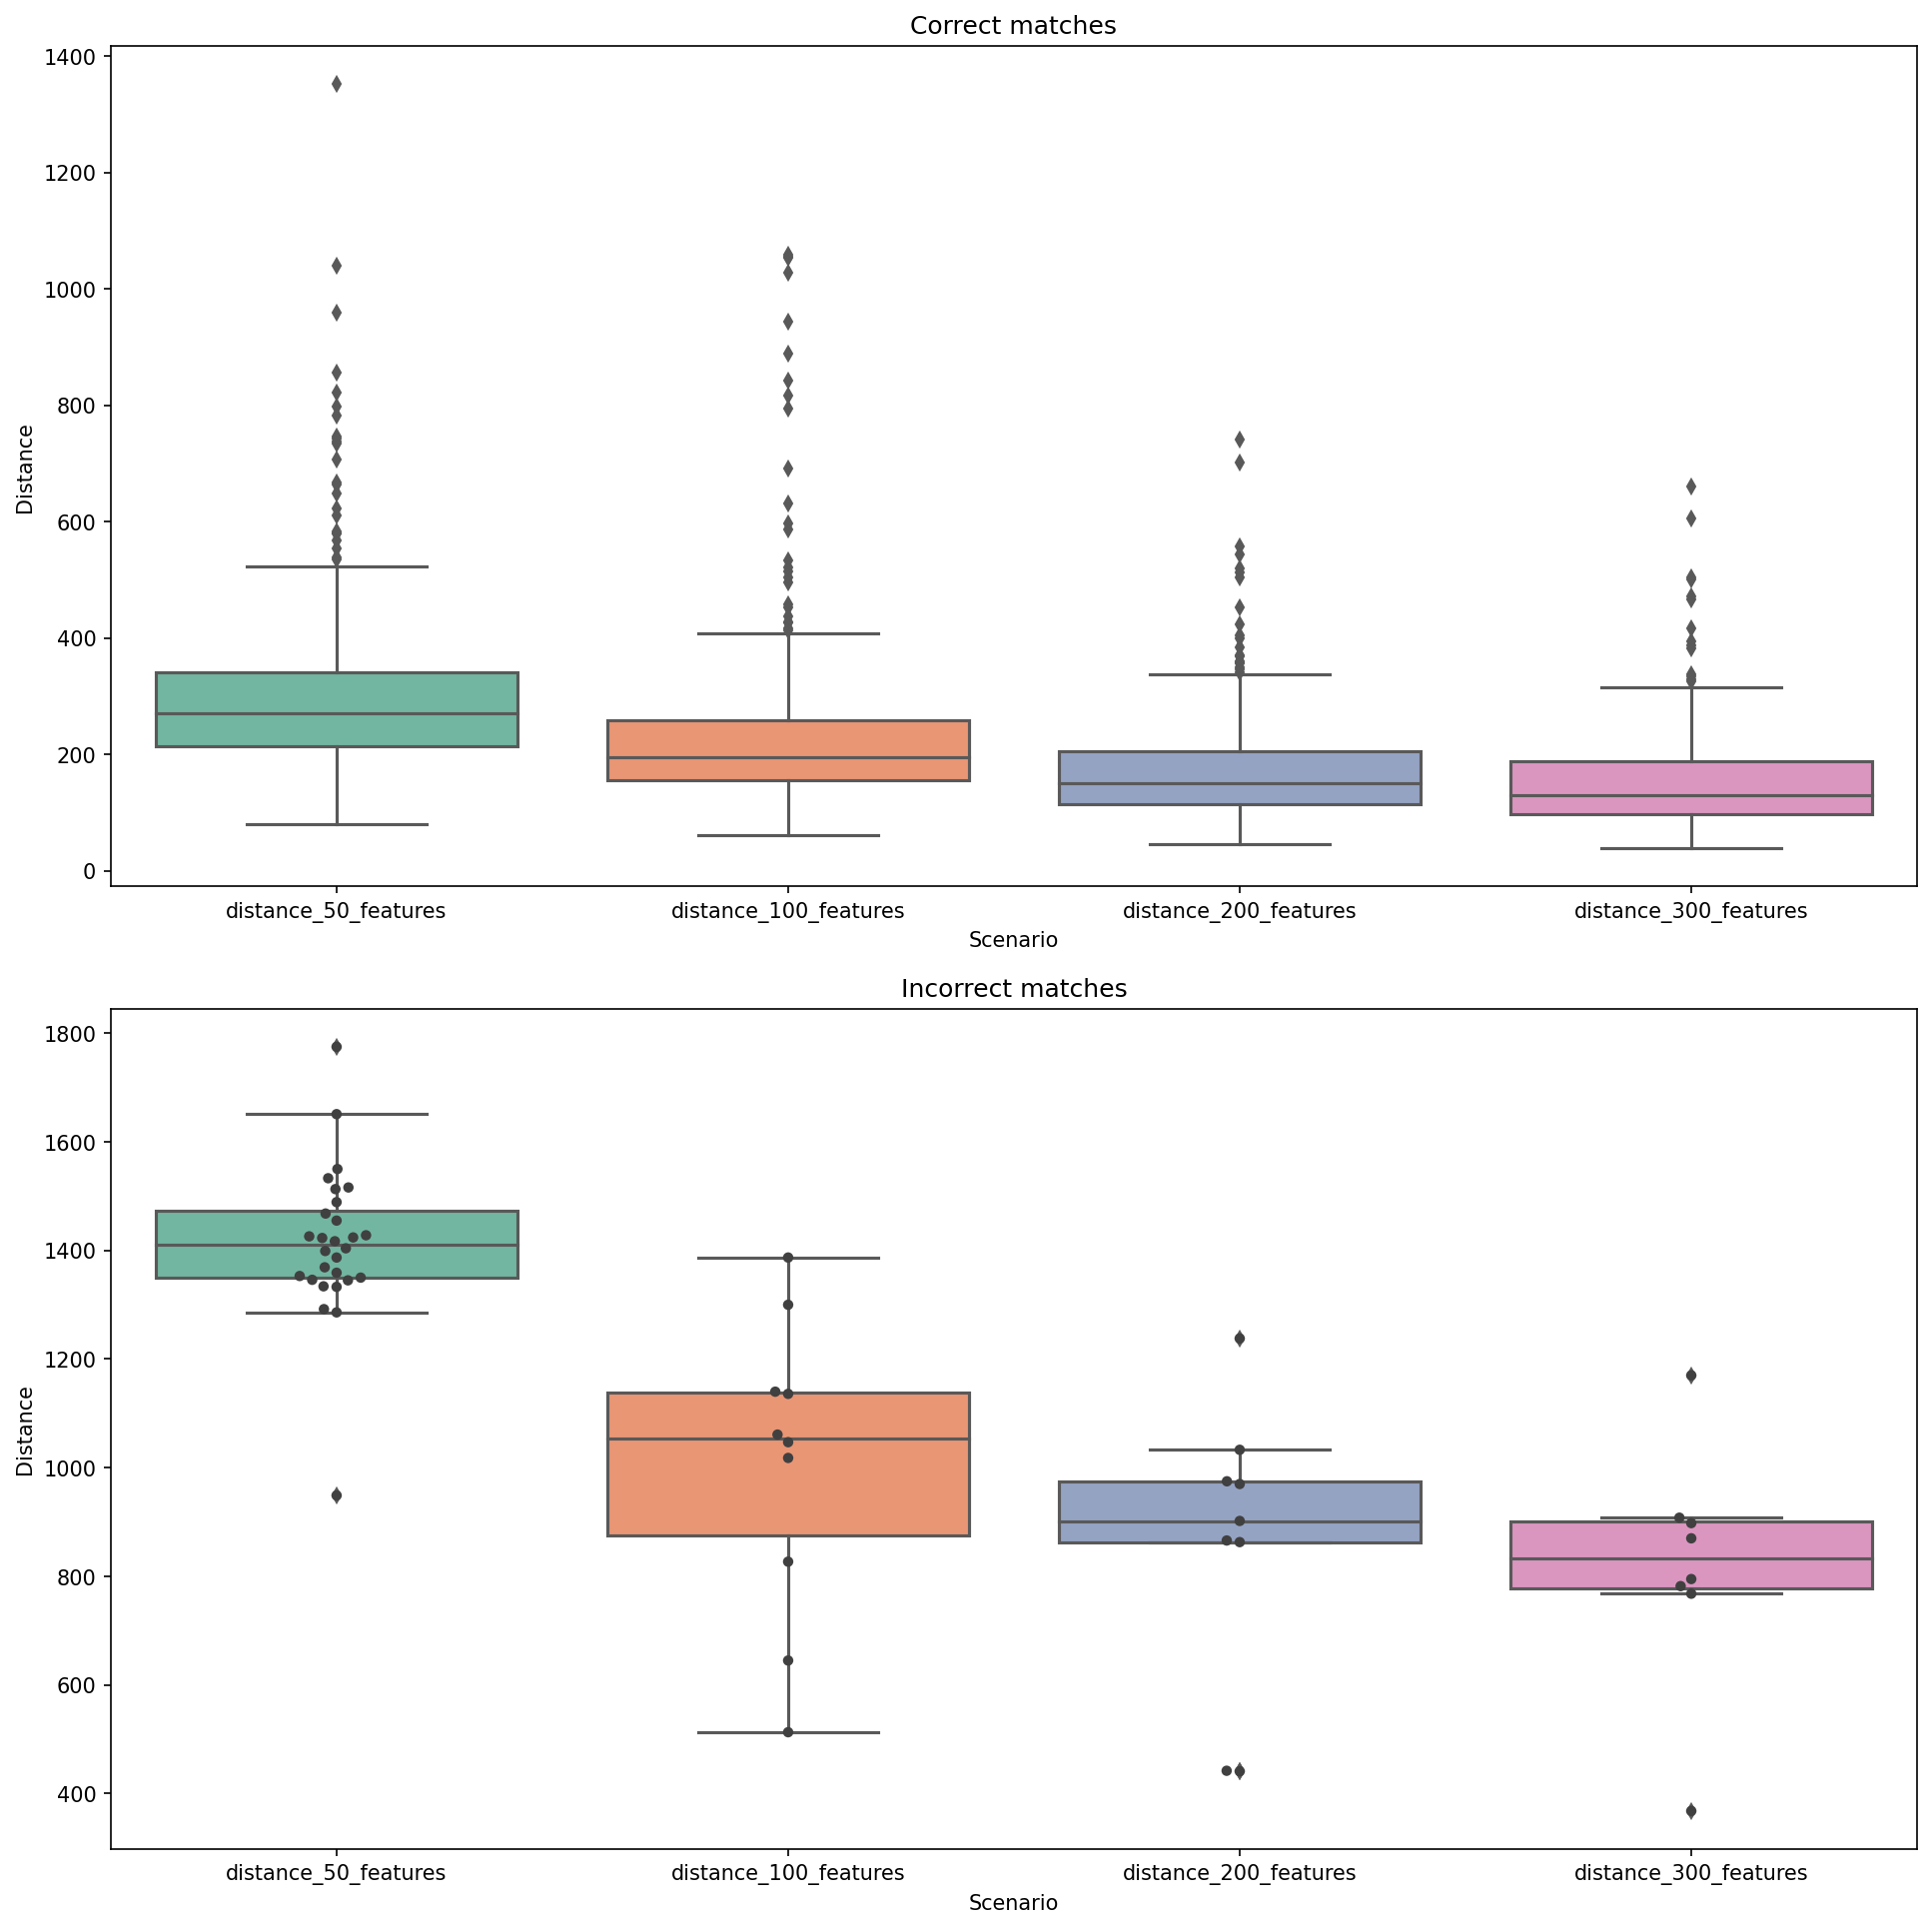
\includegraphics[width=\textwidth]{images/bxplt_distance_keypoints.png}
%     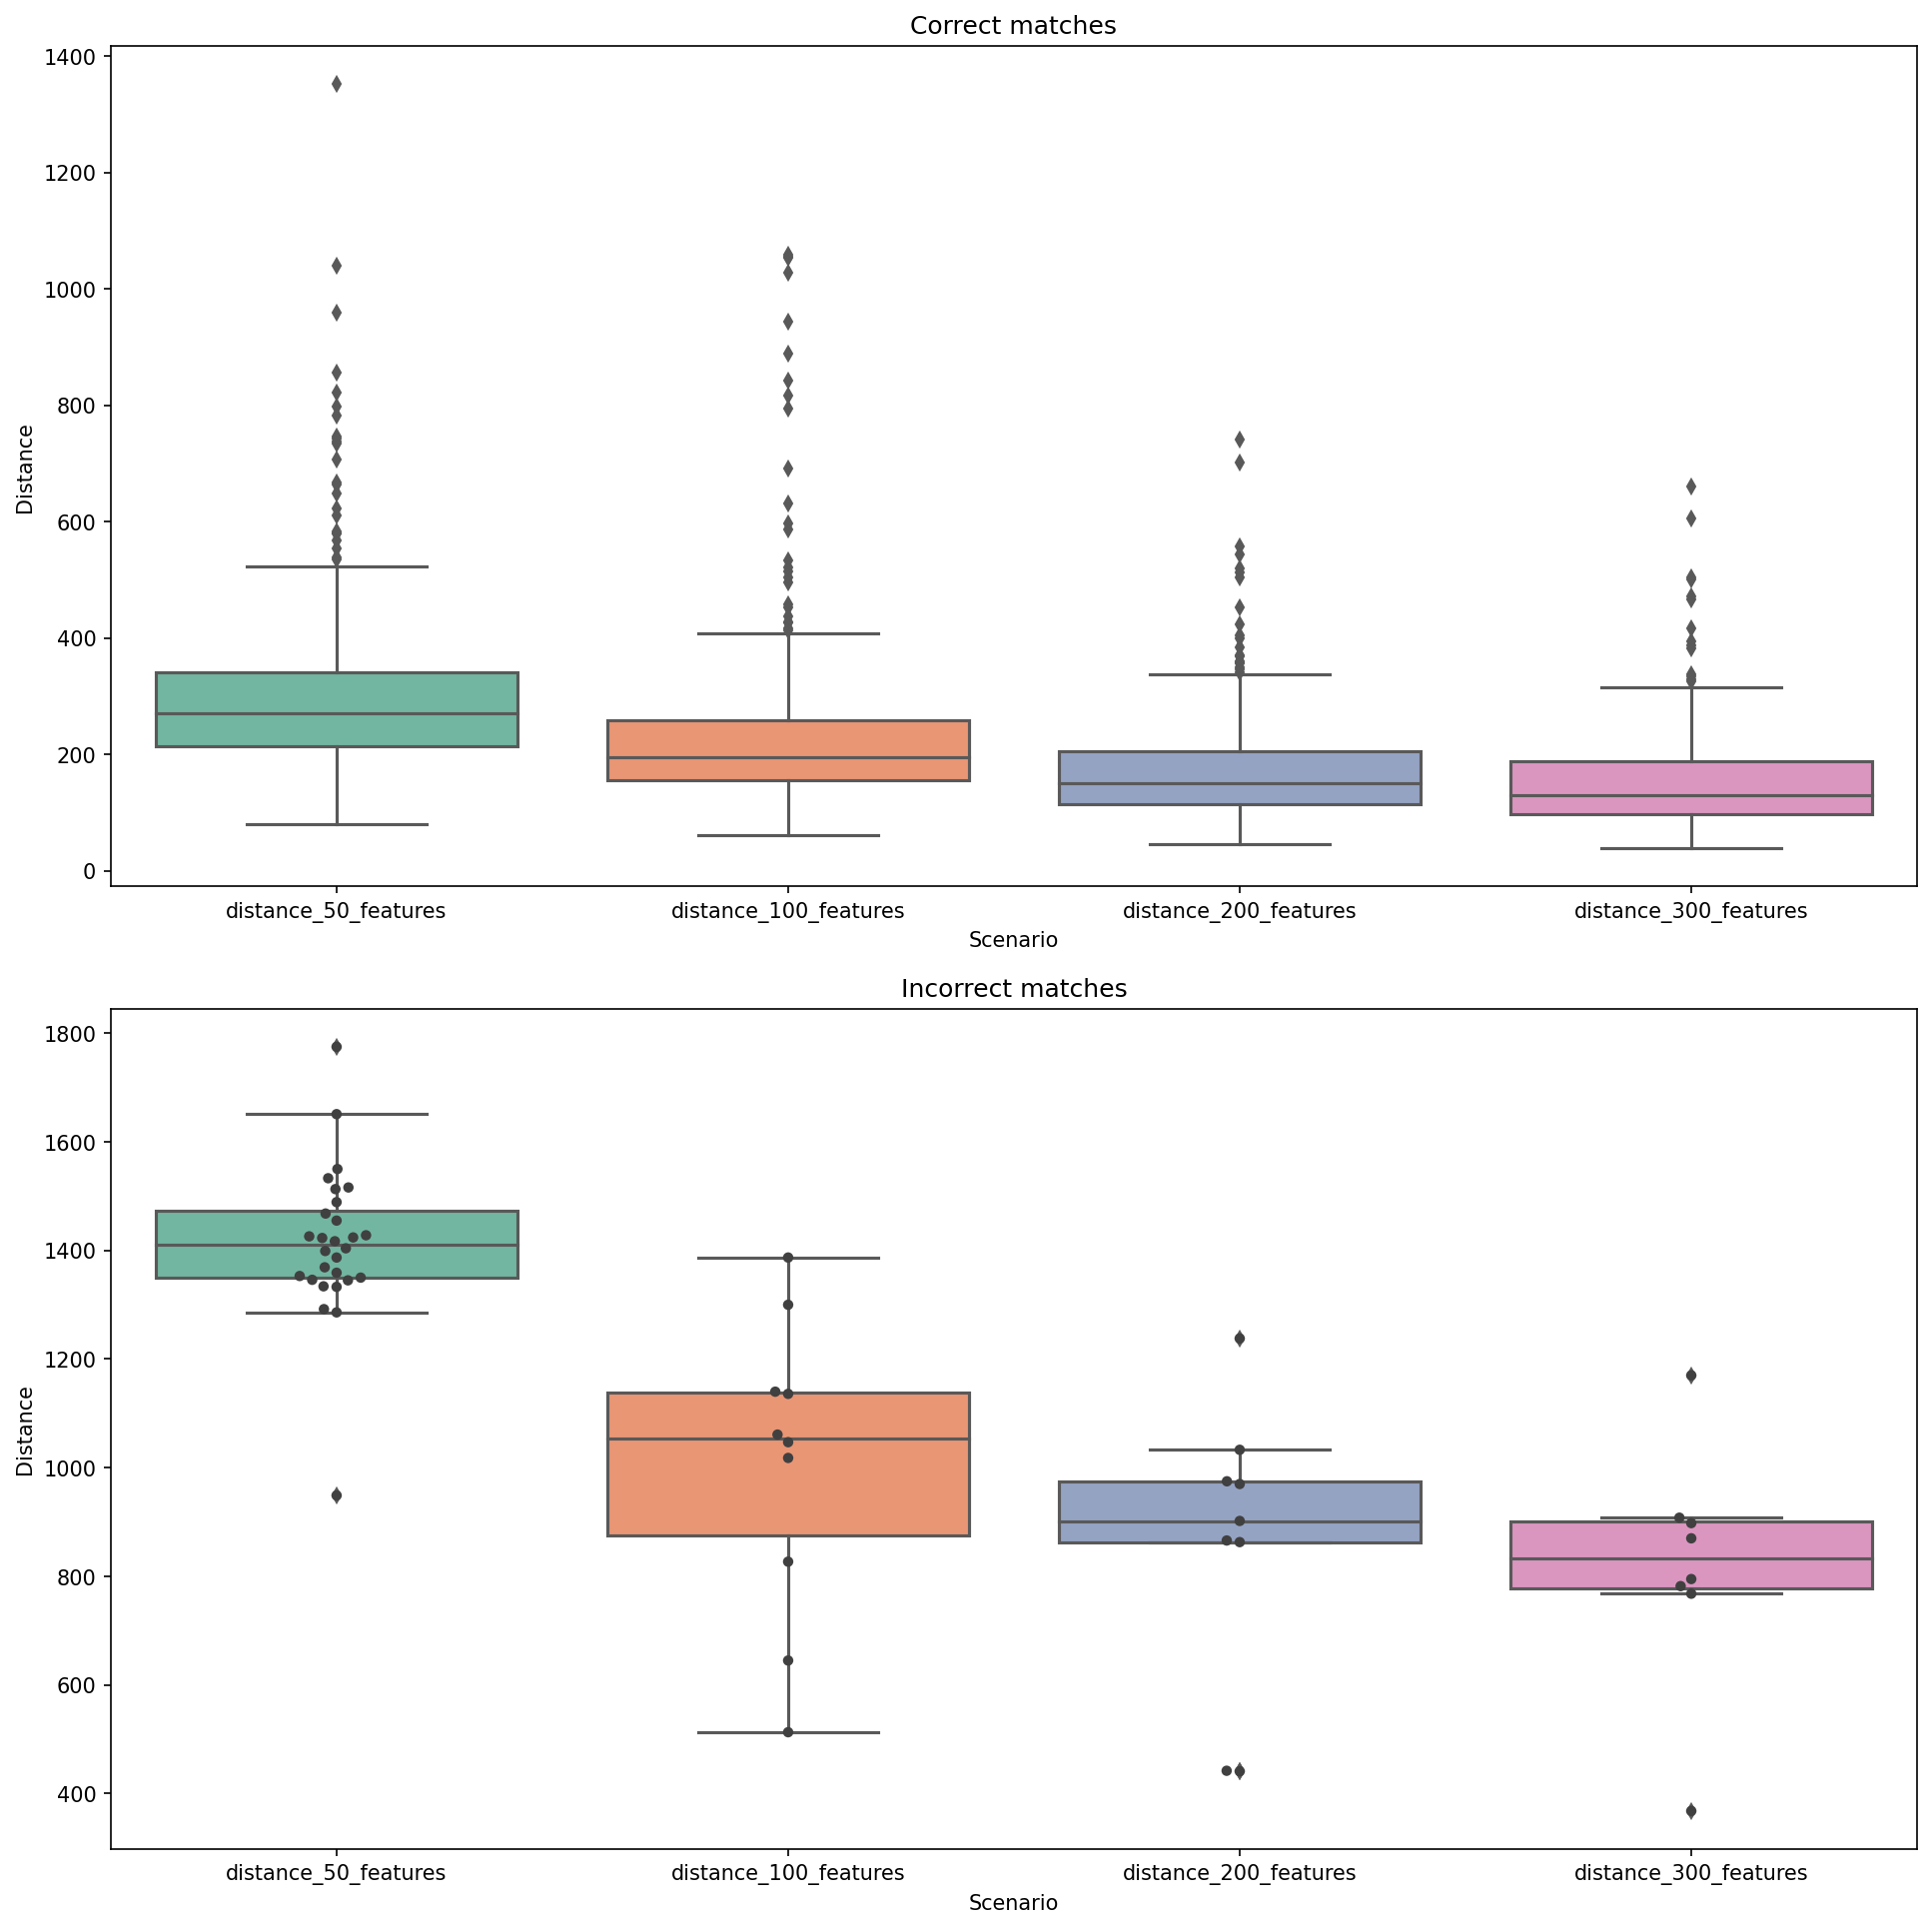
\includegraphics[width=1.6\columnwidth]{images/bxplt_distance_keypoints.png}
%     \centering
%     \caption{Distance distribution correct matches}
%     \label{fig:bxplt_distances_keypoints}
% \end{figure*}

\begin{figure}[htbp]
    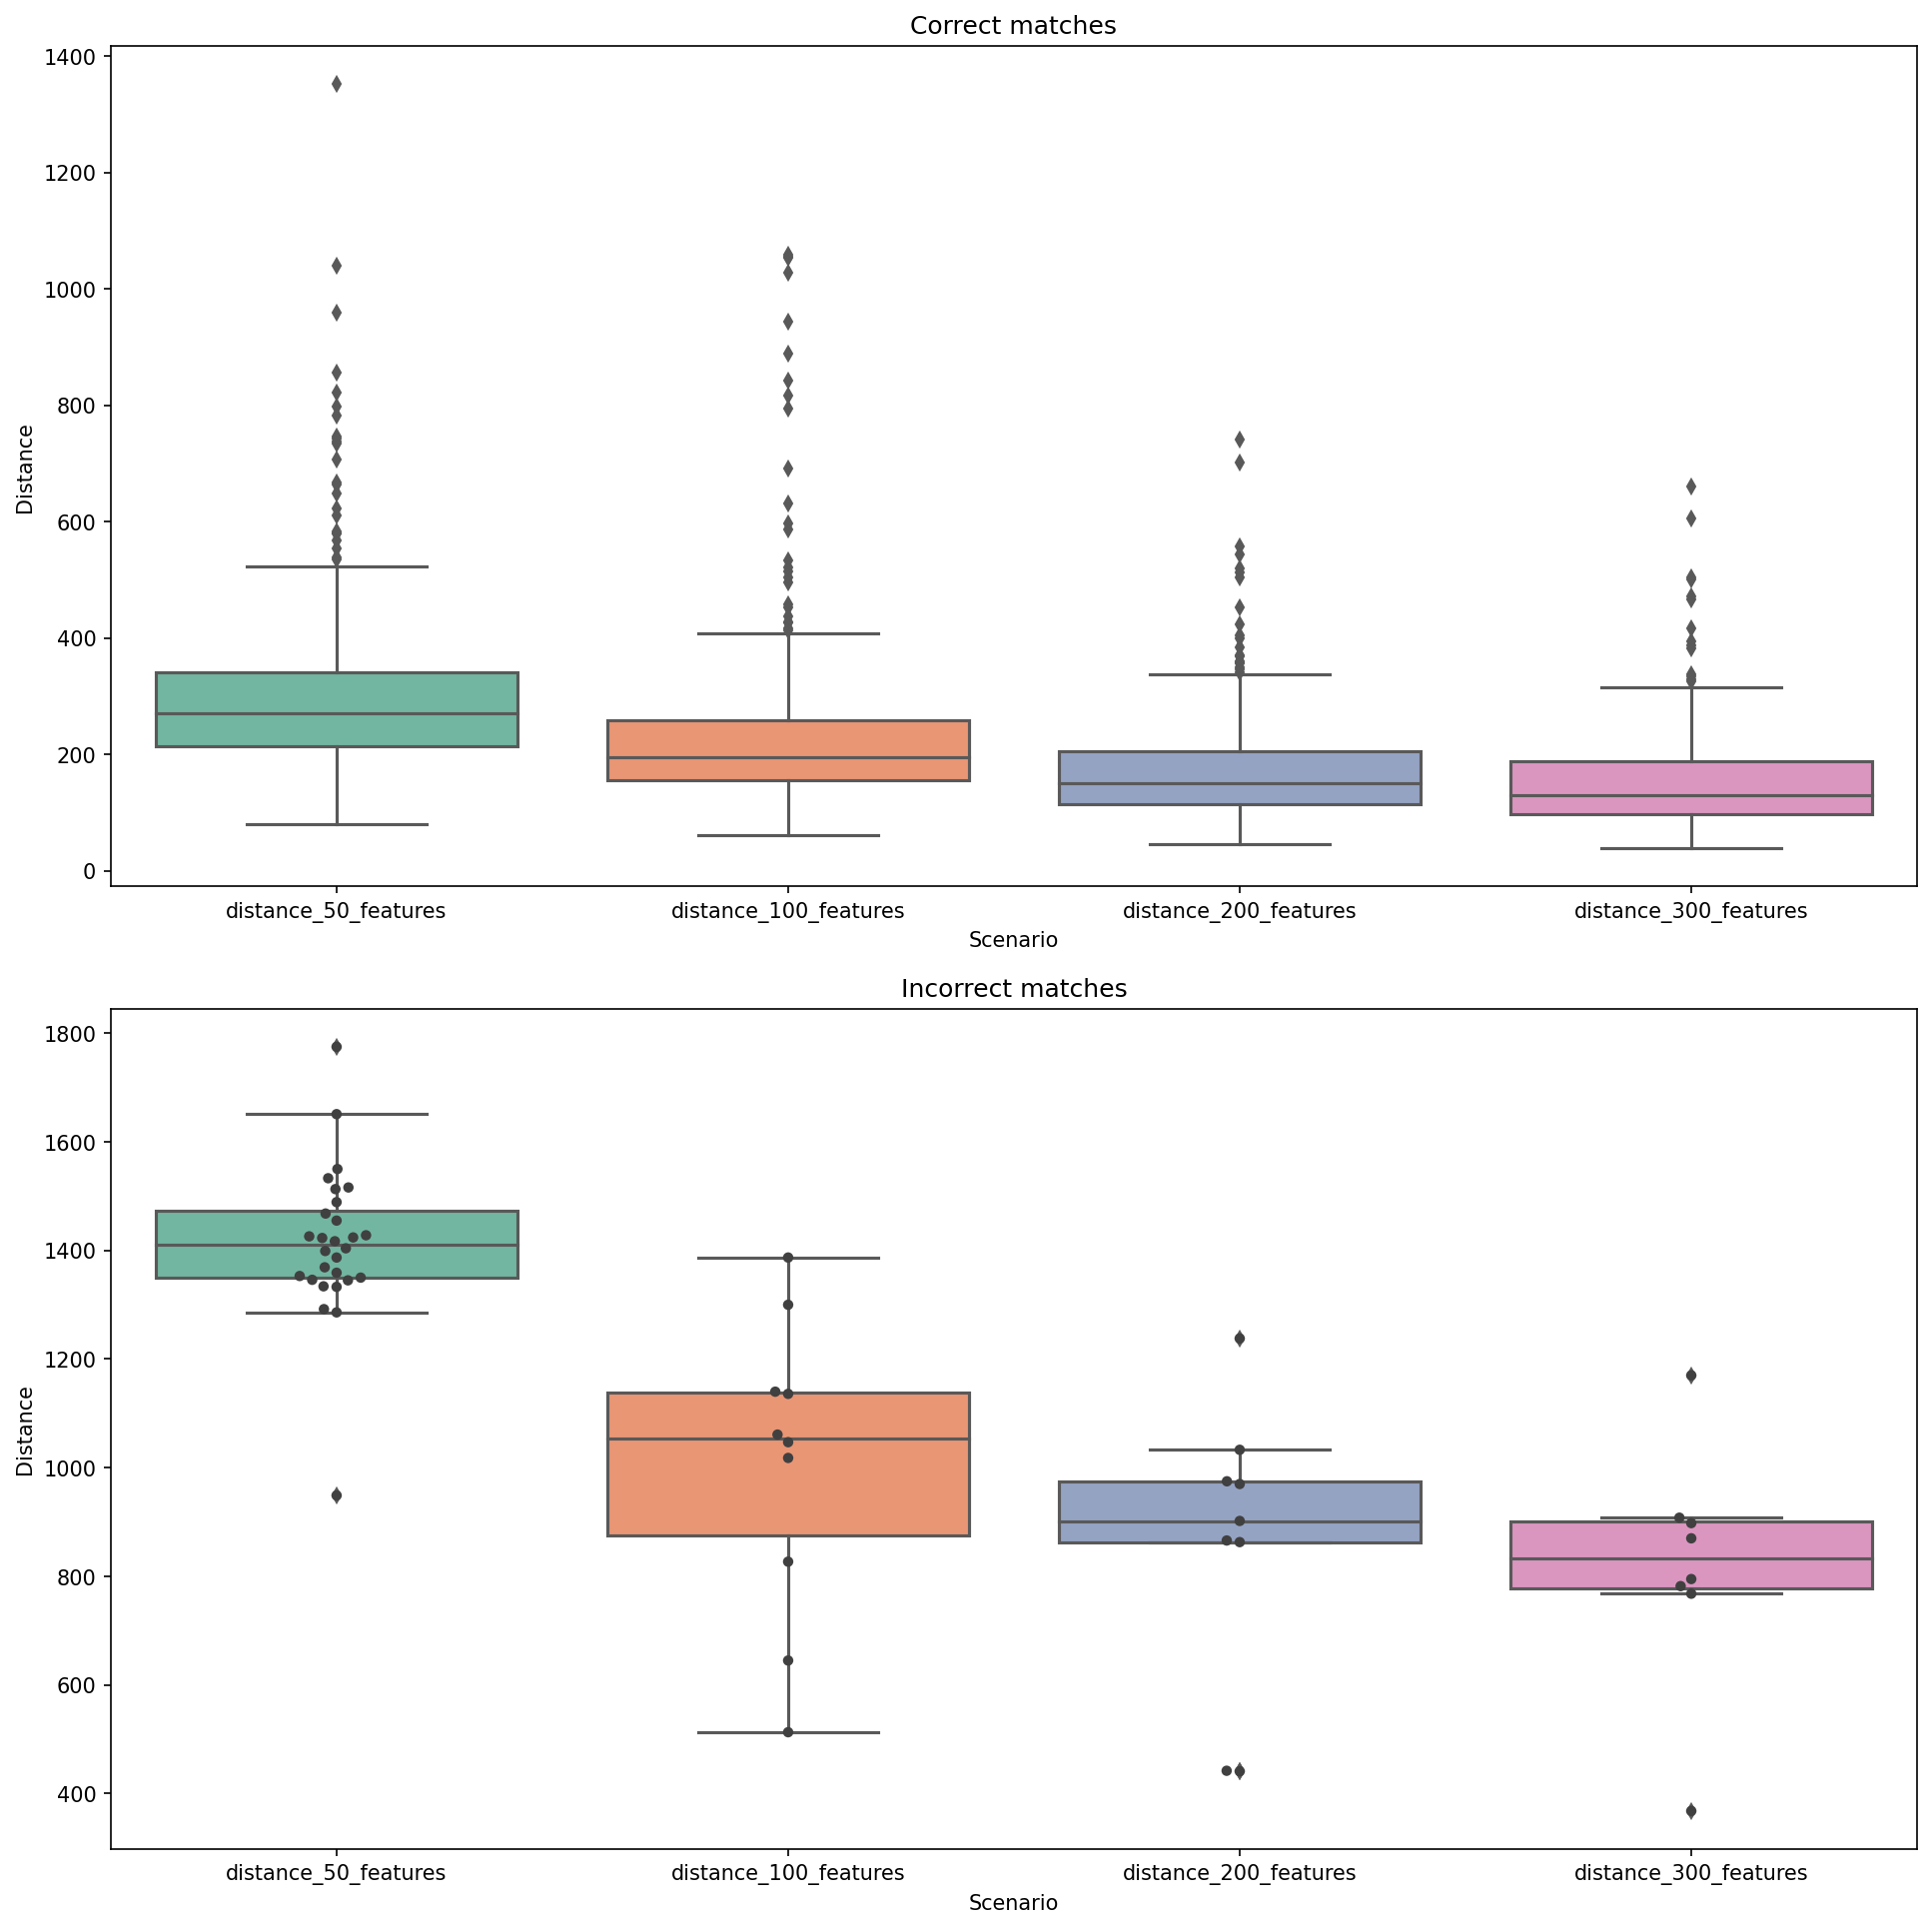
\includegraphics[width=1.0\columnwidth]{images/bxplt_distance_keypoints.png}
    \centering
    \caption{Distance distribution matches (variation of keypoints)}
    \label{fig:bxplt_distances_keypoints}
\end{figure}



\renewcommand{\arraystretch}{1.2}
\begin{table}[htbp]
    \caption{Distance distribution average values}
    \centering
    \begin{center}
        \begin{tabular}{ |c|c|c|c|  }
        %  \hline
        %  \multicolumn{4}{|c|}{Keypoint/feature variation correctness results.} \\
         \hline
         No. keypoints& Mean & Mean match & Mean no match\\
         \hline \hline
         50  & 374.98 & 302.66 & 1413.36\\
         \hline
         100 & 247.87 & 229.92 & 1007.40\\
         \hline
         200 & 187.71 & 173.47 & 858.89\\
         \hline
         300 & 164.64 & 152.30 & 819.88\\
         \hline
        \end{tabular}
    \end{center}
    \label{tab:keypoint_distance_mean}
\end{table}

Most of the wrong matched images have a strong intensity deviation or contain only dark colors. (figure \ref{fig:wrong_result_dark} and figure \ref{fig:wrong_result_light}) The effect of varying intensity is reviewed in \cite{orb_surf_sift_evaluation}. SURF and SIFT are less sensitive to this and will perform better. Nonetheless, this issue does not cause much trouble when using the videos.

\begin{figure}[htbp]
    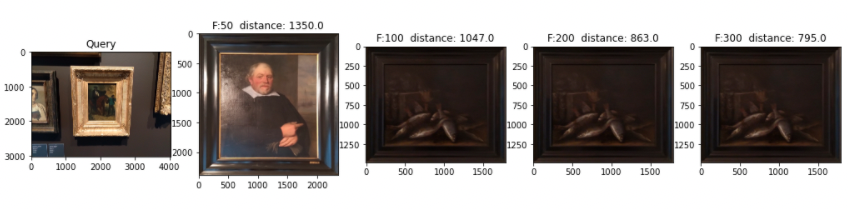
\includegraphics[width=1.0\columnwidth]{images/wrong_result cropped.png}
    \centering
    \caption{Incorrect matching results due to darkness}
    \label{fig:wrong_result_dark}
\end{figure}

\begin{figure}[htbp]
    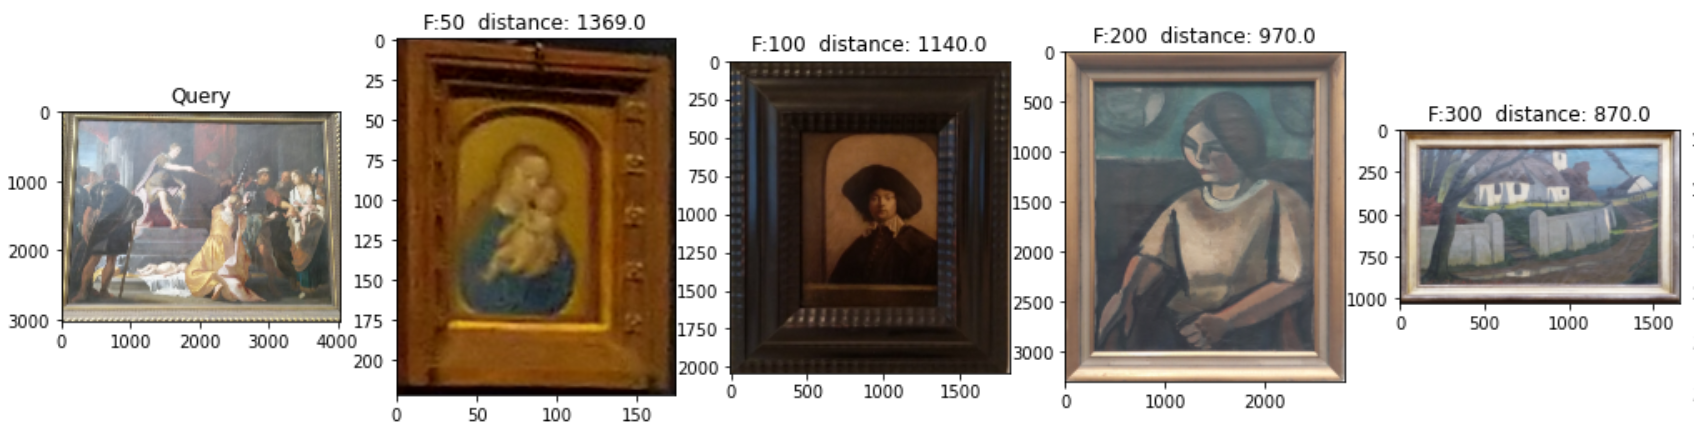
\includegraphics[width=1.0\columnwidth]{images/wrong_results_int.png}
    \centering
    \caption{Incorrect matching results due too much light}
    \label{fig:wrong_result_light}
\end{figure}

% Distance between matches

Distances between first and second matches may reflect information about the quality of a particular match. Figure \ref{fig:bxplt_difference_keypoints} confirms this assumption, the distances between the first and second matches are remarkably lower in case of incorrect matches.

% \begin{figure*}[htbp]
%     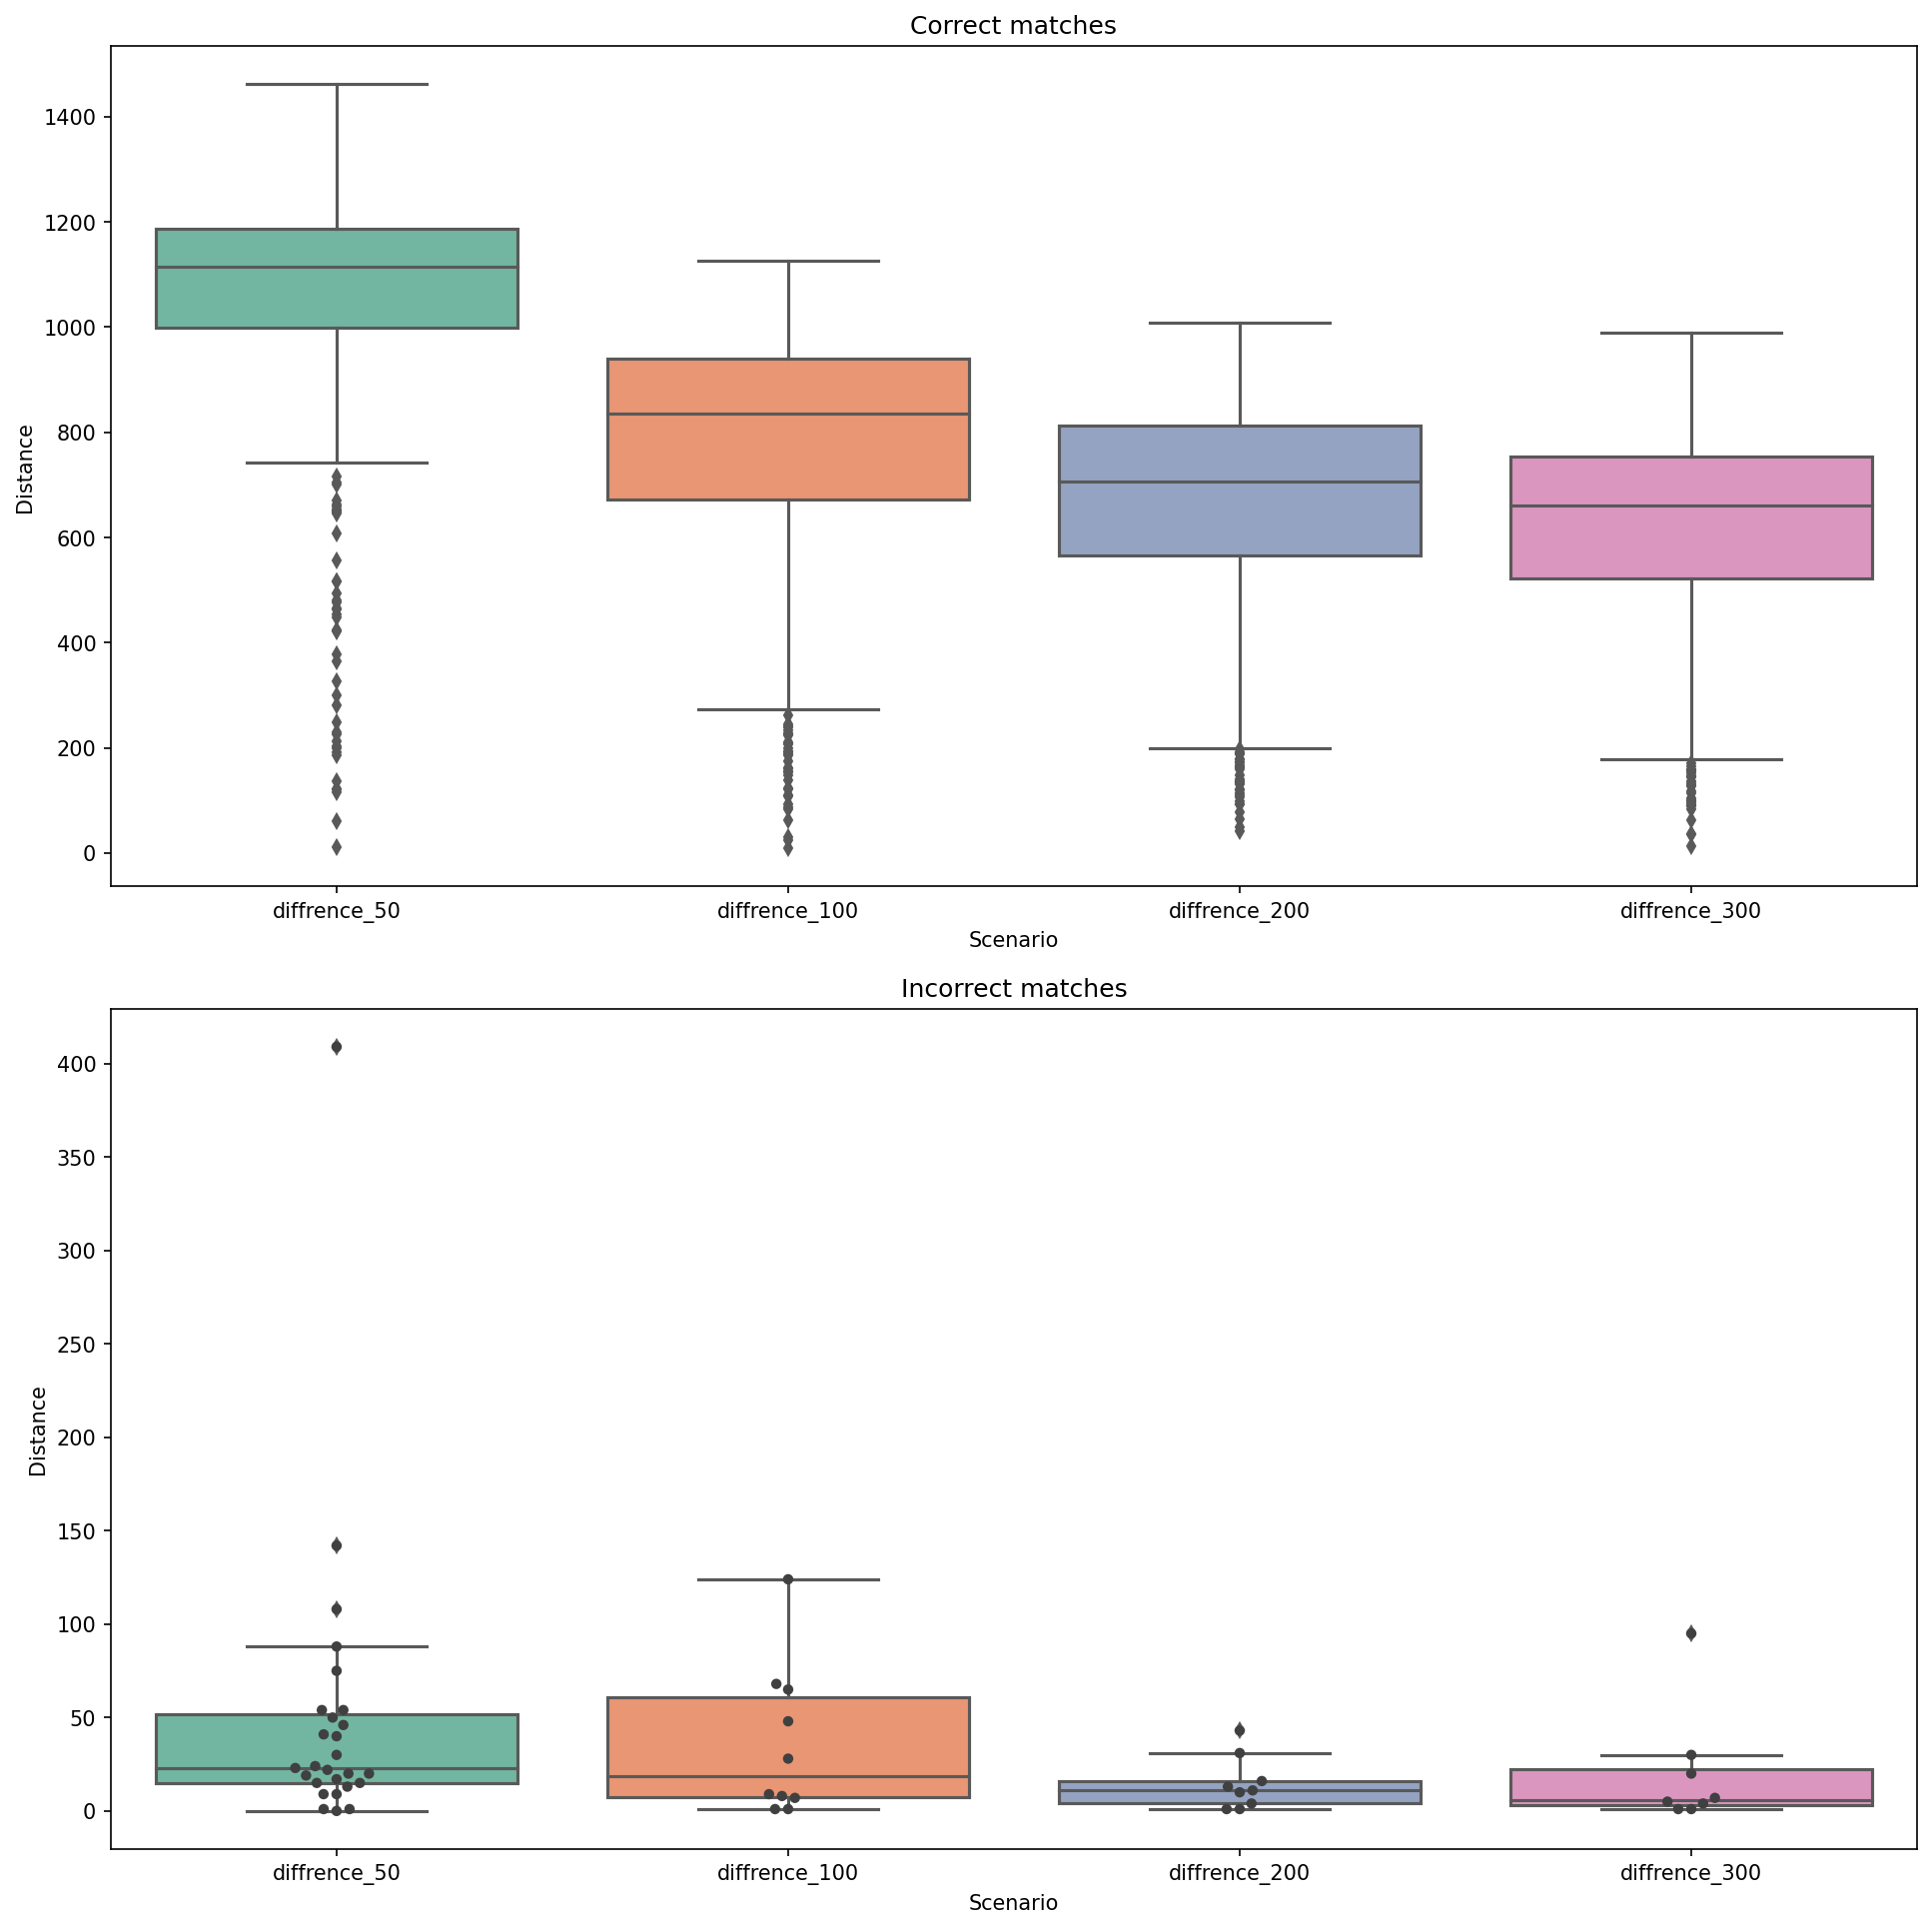
\includegraphics[width=1.6\columnwidth]{images/bxplt_difference_keypoints.png}
%     \centering
%     \caption{Difference between first and second matching result in case of correct matches}
%     \label{fig:bxplt_difference_keypoints}
% \end{figure*}

\begin{figure}[htbp]
    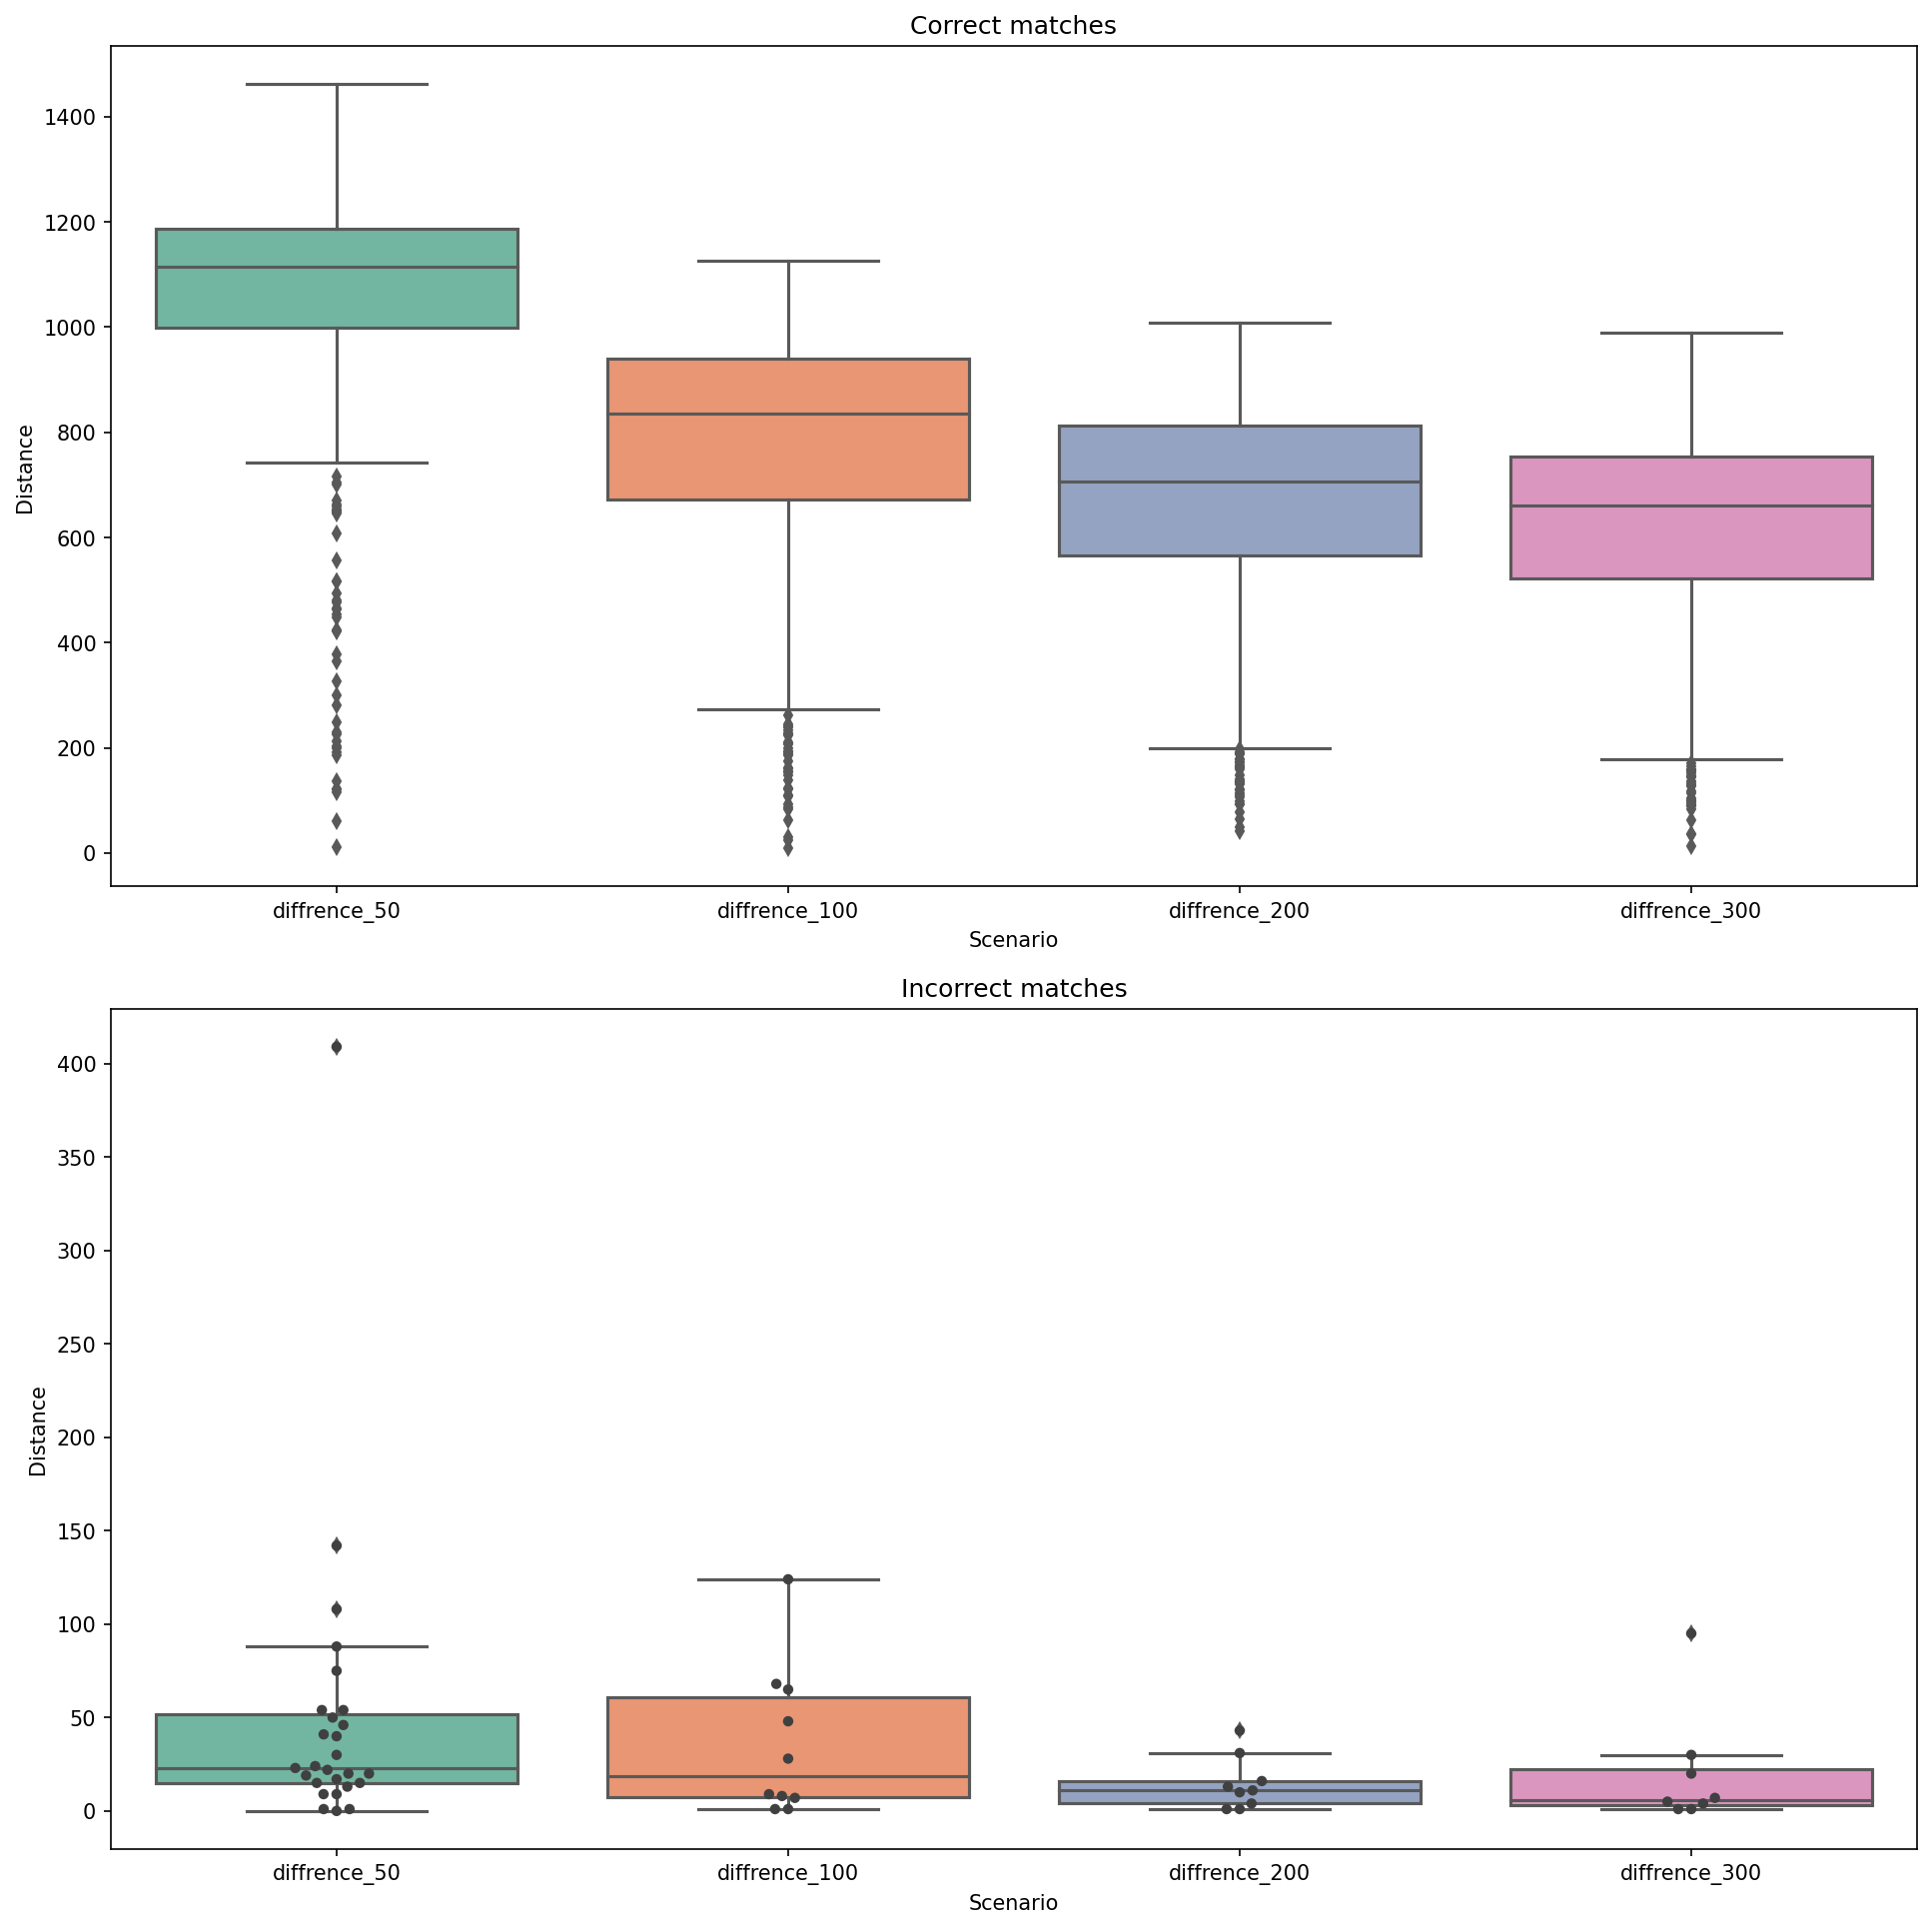
\includegraphics[width=1.0\columnwidth]{images/bxplt_difference_keypoints.png}
    \centering
    \caption{Difference in distance between the first and second matching result}
    \label{fig:bxplt_difference_keypoints}
\end{figure}

Earlier the chosen amount of keypoints/features was made on the matching score. In addition, the time to match one image is also a decisive factor. Table \ref{tab:keypoint_timing} illustrates the average time to match an image to the database. The matcher with 200 keypoints/features needs a double amount of time compared to the matcher with only 100 keypoints/features. Because of the realtime requirements, the choice for 100 keypoints is obvious.

% Time evaluation
\renewcommand{\arraystretch}{1.2}
\begin{table}[htbp]
    \caption{Keypoint/feature variation compute time}
    \centering
    \begin{center}
        \begin{tabular}{ |c|c|  }
         \hline
         No. of keypoints& Compute time (ms)\\
         \hline \hline
         50  & 60 \\
         \hline
         100 & 107 \\
         \hline
         200 & 238 \\
         \hline
         300 & 353 \\
         \hline
        \end{tabular}
    \end{center}
    \label{tab:keypoint_timing}
\end{table}

% importance of scaling
\subsection{Feature vector matching}
\label{subsec:Feature vector matching}

Our approach for feature vector matching relies on feature
extracting with a pre-trained model. The chosen model is
VGG16 with weights from imagenet. Such a model provides
interesting feature generation which is convenient for applying distance measurements \cite{feature_extraction}.

Figure \ref{fig:vgg16} illustrates all layers. The red square around the fully connected layer represents the prediction layer. This (dense) layer was cut off to obtain the feature vectors.

\begin{figure}[htbp]
    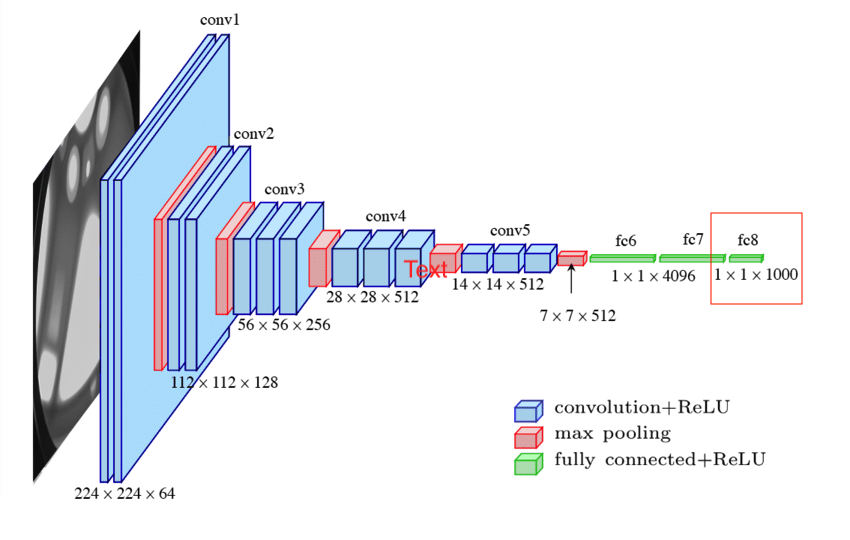
\includegraphics[width=1.0\columnwidth]{images/vgg16.png}
    \centering
    \caption{VGG16 layer visualization \cite{vgg16_image}}
    \label{fig:vgg16}
\end{figure}

Various distance metrics are applicable to obtain a distance result between the feature vectors. The following common metrics were evaluated: euclidean, cityblock, Minkowski, Chebyshev, and cosine. Table \ref{tab:fvector_score} shows the matching results on the same evaluation dataset in \ref{subsec:Keypoint matching}. Euclidean seems to have the highest positive ratio. The cityblock and cosine metrics also have acceptable scores. Only Chebyshev scores substandard.

%https://pdodds.w3.uvm.edu/research/papers/others/everything/cha2007a.pdf

\renewcommand{\arraystretch}{1.2}
\begin{table}[htbp]
    \caption{Distance metric variation correctness results}
    \centering
    \begin{center}
        \begin{tabular}{ |c|c|c|c|  }
         \hline
         Metric& Positive matches &Negative matches&Mean score (\%)\\
         \hline \hline
         euclidean & 363 & 74 & 83.07\\
         \hline
         cityblock & 358 & 79 & 81.92\\
         \hline
         chebyshev & 315 & 122 & 72.08\\
         \hline
         cosine & 360 & 77 & 82.38\\
         \hline
        \end{tabular}
    \end{center}
    \label{tab:fvector_score}
\end{table}

Each distance metric results in another range of distance values. (Table \ref{tab:fvector_distance_mean}) Comparing the correct matches distribution with the incorrect matches, an overlapping region is established for each distance metric.

\renewcommand{\arraystretch}{1.2}
\begin{table}[htbp]
    \caption{Distance distribution average values}
    \centering
    \begin{center}
        \begin{tabular}{ |c|c|c|c|  }
        %  \hline
        %  \multicolumn{4}{|c|}{Keypoint/feature variation correctness results.} \\
         \hline 
         Metric& Mean & Mean match & Mean no match\\
         \hline \hline
         euclidean  & 49.70 & 302.66 & 1413.36\\
         \hline
         cityblock & 1420.49 & 1371.98 & 1640.33\\
         \hline
         chebyshev & 5.22 & 5.16 & 5.38\\
         \hline
         cosine & 0.16 & 0.14 & 0.24\\
         \hline
         \end{tabular}
    \end{center}
    \label{tab:fvector_distance_mean}
\end{table}

Despite this property, differences between the first and second matches are still useful. The mean values for the differences between the first and second matches are shown in table \ref{tab:fvector_difference_mean}.

\renewcommand{\arraystretch}{1.2}
\begin{table}[htbp]
    \caption{Difference in distance distribution average values}
    \centering
    \begin{center}
        \begin{tabular}{ |c|c|c| }
        %  \hline
        %  \multicolumn{4}{|c|}{Keypoint/feature variation correctness results.} \\
         \hline
         Metric& Mean match & Mean no match\\
         \hline \hline
         euclidean  & 11.64 & 1.78\\
         \hline
         cityblock & 356.85 & 54.80\\
         \hline
         chebyshev & 1.02 & 0.22\\
         \hline
         cosine & 0.08 & 0.02 \\
         \hline
        \end{tabular}
    \end{center}
    \label{tab:fvector_difference_mean}
\end{table}

% \begin{figure}[htbp]
%     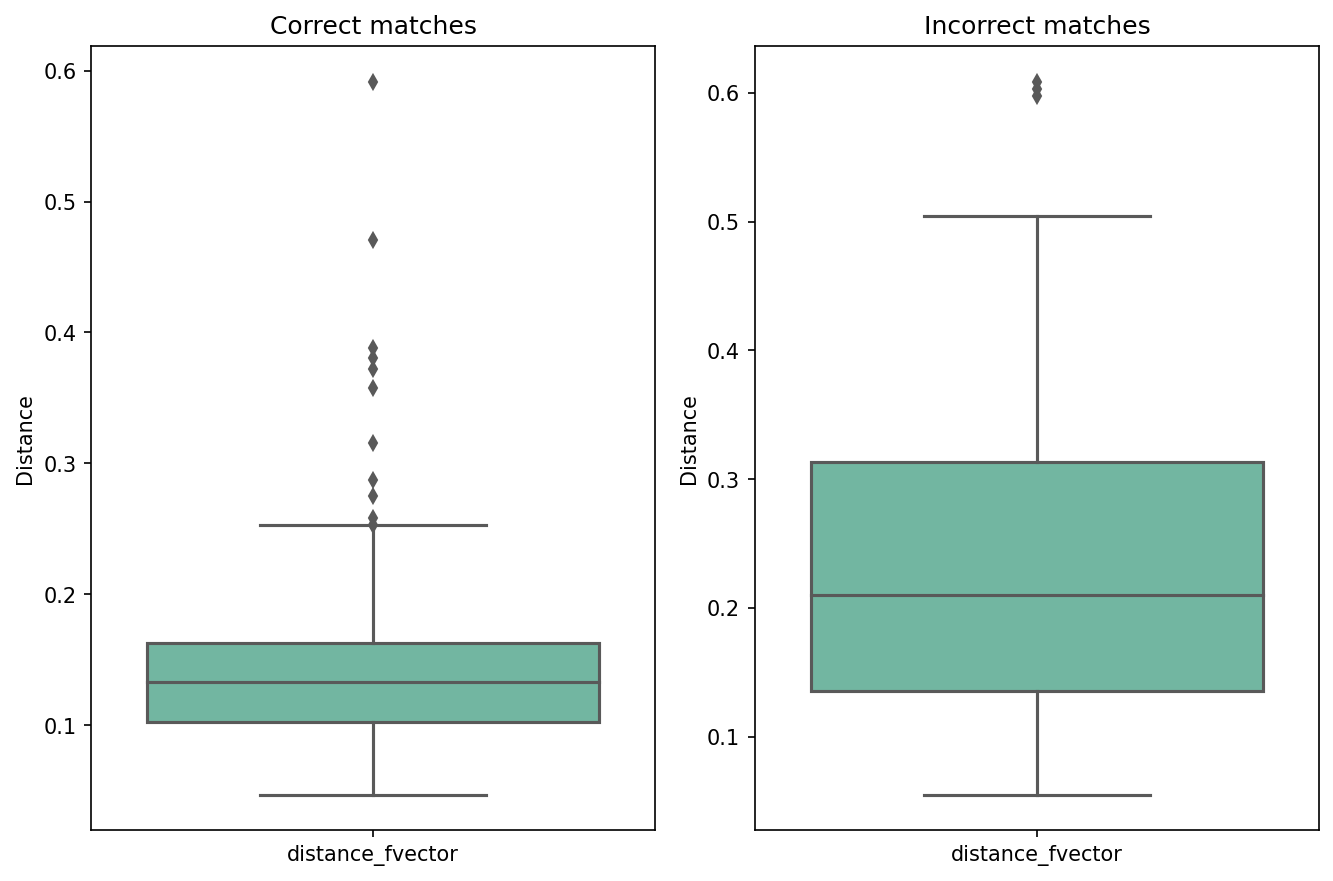
\includegraphics[width=0.8\columnwidth]{images/bxplt_distance_fvectors.png}
%     \centering
%     \caption{Distance distribution, left: correct matches | right: incorrect matches}
%     \label{fig:bxplt_distances_fvector}
% \end{figure}

% \begin{figure}[htbp]
%     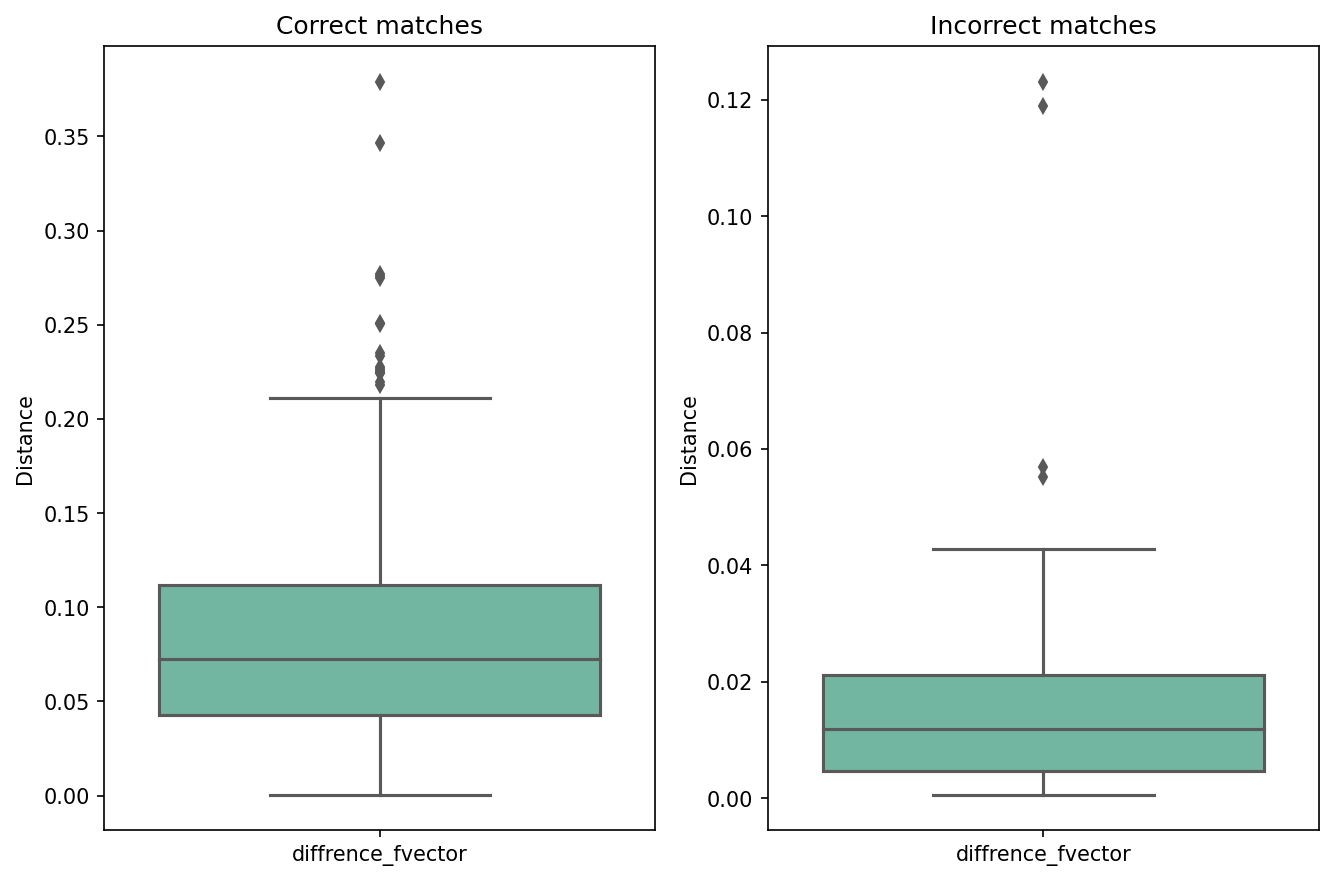
\includegraphics[width=0.8\columnwidth]{images/bxplt_difference_fvectors.png}
%     \centering
%     \caption{Difference between first and second matching result, left: correct matches | right: incorrect matches}
%     \label{fig:bxplt_diffrences_fvector}
% \end{figure}


Next to these distance and matching scores, time should also be taken into account when choosing a suitable distance metric. Table \ref{tab:fvector_timing} illustrates the average time to match an image upon the database. The matcher using the cityblock metric seems to have the fastest execution, followed by euclidean and cosine. The chebyshev version scores substandard again.

Based on the collected results euclidean and cityblock are the better choices. Both distance metrics are used to demonstrate the effects on the videos.

% Time evaluation
\renewcommand{\arraystretch}{1.2}
\begin{table}[htbp]
    \caption{Compute time distance metric dependent}
    \centering
    \begin{center}
        \begin{tabular}{ |c|c|  }
         \hline
         Distance metric& Compute time (ms)\\
         \hline \hline
         euclidean & 69.60\\
         \hline
         cityblock & 54.87\\
         \hline
         chebyshev & 221.30\\
         \hline
         cosine & 77.15\\
         \hline
        \end{tabular}
    \end{center}
    \label{tab:fvector_timing}
\end{table}

% distance pictures


\subsection{Matching evaluation}
\label{subsec:Matching evaluation}

All collected metrics for both matching approaches result in three final matchers which can be used in the realtime application: the keypoint-based matcher with 100 keypoints/features, the feature vector-based matching with euclidean distance metric, and the feature vector-based matching with cityblock distance metric.

The feature vector-based matchers have a faster compute time than the keypoint-based matcher while the keypoint-based matcher is more reliable in terms of correct matching. Because of this reason next to the implementations where only one kind of matcher is used, we also added a combination of a feature vector and a keypoint-based matcher.

This implementation takes advantage of the speed of the feature vector-based matcher. The matcher returns the first 50 images that may be a match. Next, the keypoint-based matcher only uses the 50 images which were returned by the feature vector-based matcher. The matching time for the keypoint-matcher is strongly reduced because only 50 images are considered instead of the whole database.

In general, one can conclude that the matching works well. It scores high when evaluating the dataset. In practice, as quoted before, blurry images and variant intensity caused by video usage still have an influence that cannot be ignored.
\section{Localisation}
\label{sec:localisation}

Now that we can extract a matching score from the paintings, we can use this to deduce the room we're currently in. If we only use the matching score our room prediction would be very heavily influenced by possible mismatches. This is why we opted for the use of a hidden Markov model (HMM).

\subsection{Hidden Markov Model}
A hidden Markov model is a statistical model that can combine the matching score with spatio-temporal features to become a room prediction. This is perfect for our assignment because, as stated previously, a prediction that's only based on the matching score would be very dependent on the quality of the matching algorithm which would make it very susceptible to mismatches.

\subsubsection{Architecture}
The underlying architecture of a HMM consists of 2 layers, a hidden layer and a layer with observed variables. The hidden layer consists of the transition probabilities between different states. The observed variables are observations that belong to a certain state with a certain probability. In this project, these "states" represent the different rooms, while the transition probability stands for the probability that a person stays in the current room or goes from the current room to another room. The processed video frames are the observed variables, where the probability of this frame belonging to a certain state/room is calculated by using the matching score of multiple matches. An example of the hidden Markov model architecture is shown in figure \ref{fig:hmm}.


\begin{figure}[htbp]
    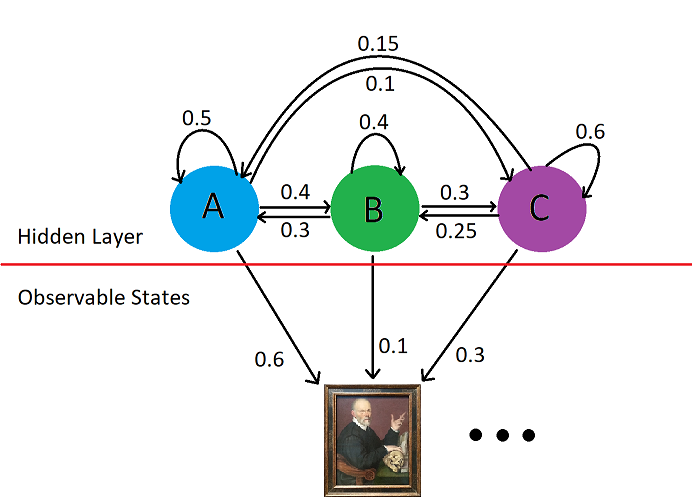
\includegraphics[width=\linewidth]{images/hmm.png}
    \caption{Hidden Markov Model architecture}
    \label{fig:hmm}
\end{figure}

\subsubsection{Calculating the transition probabilities}
The amount of rooms between the start and destination room is used as a metric to calculate the transition probabilities between the rooms. If there are more rooms between the two rooms, the probability of the next frame being in the destination room would be lower than when the start and destination room would be adjacent. The reasoning behind this is pretty straightforward. It’s simply very unlikely that a person goes from a certain room to the other side of the museum in a matter of seconds.
To apply this in our program, we first need to know the number of rooms that are between the start and destination room. Note that we only have the floor plan of the museum to start with. Starting from this floor plan, an undirected graph was created where the connected nodes represent the adjacent rooms. After creating this graph, we extract the adjacency matrix to become a matrix structure that shows the adjacent rooms.
From this adjacency matrix, we can calculate the distance matrix by using the Floyd Warshall algorithm \cite{floyd_warshall}, which is an algorithm that’s used to calculate the optimal path between all the different nodes in a graph.
Now that the distance matrix is calculated, a distribution has to be applied to the rows which makes sure that the shortest distances have the highest probability, while the longest distances have the lowest probability. For this project, a linear and a Gaussian distribution were created and after extensive testing, the Gaussian distribution with $\mu = 0$ and $\sigma = 1$ was found to be the best performing distribution. \par 
The process to create the transition probabilities is visualized below for the example in fig. \ref{fig:hmm} where we assume that the rooms are in a straight line (A - B - C). We start from the connectivity matrix, to become the distance matrix and end up with the probability matrix after applying the Gaussian distribution.

\[
\begin{bNiceMatrix}[first-row,first-col]
  & A & B & C \\
A & 0 & 1 & 0 \\
B & 1 & 0 & 1 \\
C & 0 & 1 & 0 
\end{bNiceMatrix} 
\Rightarrow
\begin{bmatrix}
0 & 1 & 2 \\
1 & 0 & 1 \\
2 & 1 & 0 \\
\end{bmatrix}
\Rightarrow
\begin{bmatrix}
0,58 & 0.35 & 0.07 \\
0.27 & 0.46 & 0.27 \\
0.07 & 0.35 & 0.58 \\
\end{bmatrix}
\]

%\begin{figure}[htbp]
%    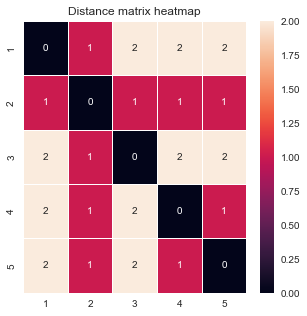
\includegraphics[width=\linewidth]{images/distance_matrix_5x5.png}
%    \caption{Distance Matrix HMM (5x5)}
%    \label{fig:distance_matrix_5x5}
%\end{figure}

\subsubsection{Calculating the probabilities for the observable variables}
Next up,  the probabilities for the observable variables have to be calculated. The observable variables in the HMM are the frames that are effectively processed and matched against the database. The probabilities are calculated based on the matching scores (distance with ORB) from the extracted contours.
The algorithm goes as follows:
For every extracted contour, the best matching score (lowest = best) is taken for each possible room based on the list of soft matches from that contour. The room scores for every room are then added together. Based on this list of scores for every room, the probability is calculated so the lowest score gets the highest probability and similar scores get similar probabilities. To reduce the effect of mismatches, the probability of the previous room is set to 2\% if there are no soft matches for that room.
\\
\subsubsection{Making the room prediction}
To make the room prediction, the transition probabilities are combined with the probabilities for the observable variables.
For every room, the probability is calculated by using the forward algorithm \cite{blunsom2004hidden} \cite{ahmadian2018systematic}, which is a dynamic algorithm that uses the following formula to calculate the probability of the frame being in a certain room $\alpha_t(x_t)$.  \[ \alpha_t(x_t) = p(y_t|x_t) \sum_{x_{t-1}}p(x_t|x_{t-1})\alpha_{t-1}(x_{t-1}) \] 
This formula simply calculates the chance that the current frame is in a certain room, based on the probabilities for each room in the previous frame $p(x_t|x_{t-1})\alpha_{t-1}(x_{t-1})$. The room probabilities based on the matching score alone are represented as $p(y_t|x_t)$. When processing the first frame no previous prediction exists. Therefore, the stationary distribution $\pi$ is used for the first frame. The stationary distribution represents the row vector such that $\pi = \pi P$, where $P$ represents the hidden layers of the model. By using this, we become starting probabilities where the rooms with more neighbors get a higher probability.\par

After applying the forward algorithm, the location prediction is obtained by simply selecting the room with the highest probability.


\subsection{Hidden Markov Model visualization}

The room predictions from the hidden Markov model are extracted and used to color-code a floor plan of MSK Ghent (see figure \ref{fig:hmm-viz}). Every room is assigned to a color between red and green where the colors correspond to a low, respectively high percentage of currently being in that room. The top three predictions of the most likely rooms are also displayed in the bottom-left part of the image with the prediction percentage. 
The rooms with the highest percentages in time are also connected with lines to show the traveled path on the floor plan of MSK Ghent.

\begin{figure}[htbp]
    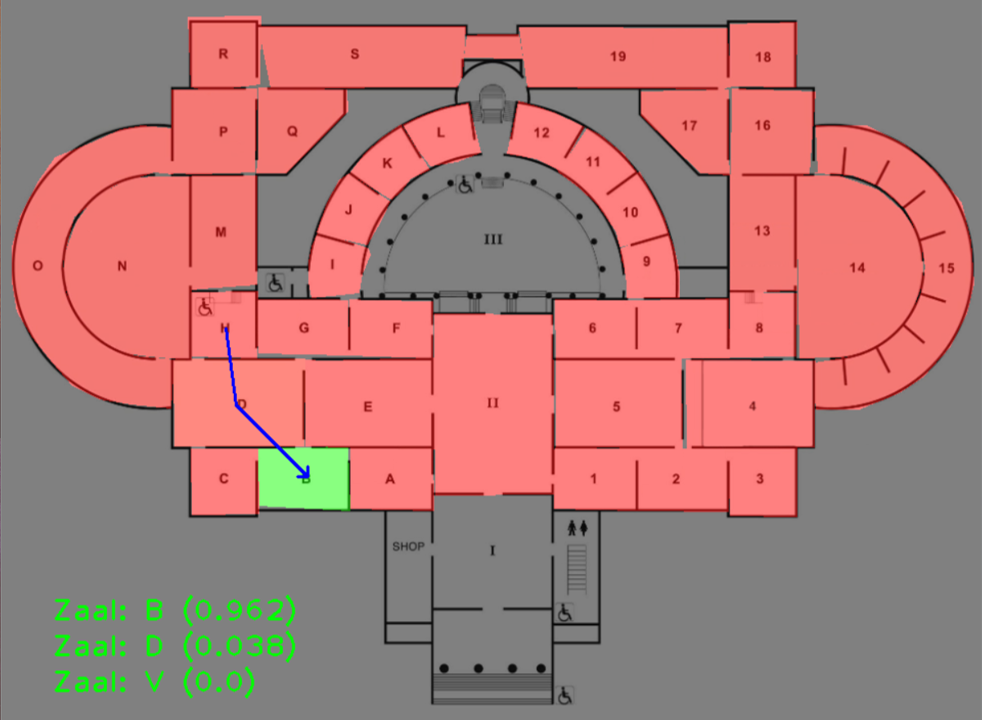
\includegraphics[width=\linewidth]{images/hmm-vis.png}
    \caption{Hidden Markov Model visualization}
    \label{fig:hmm-viz}
\end{figure}

\section*{Conclusion}

\begin{figure*}
	\centering
	\begin{minipage}{1.5\columnwidth}
		\centering
		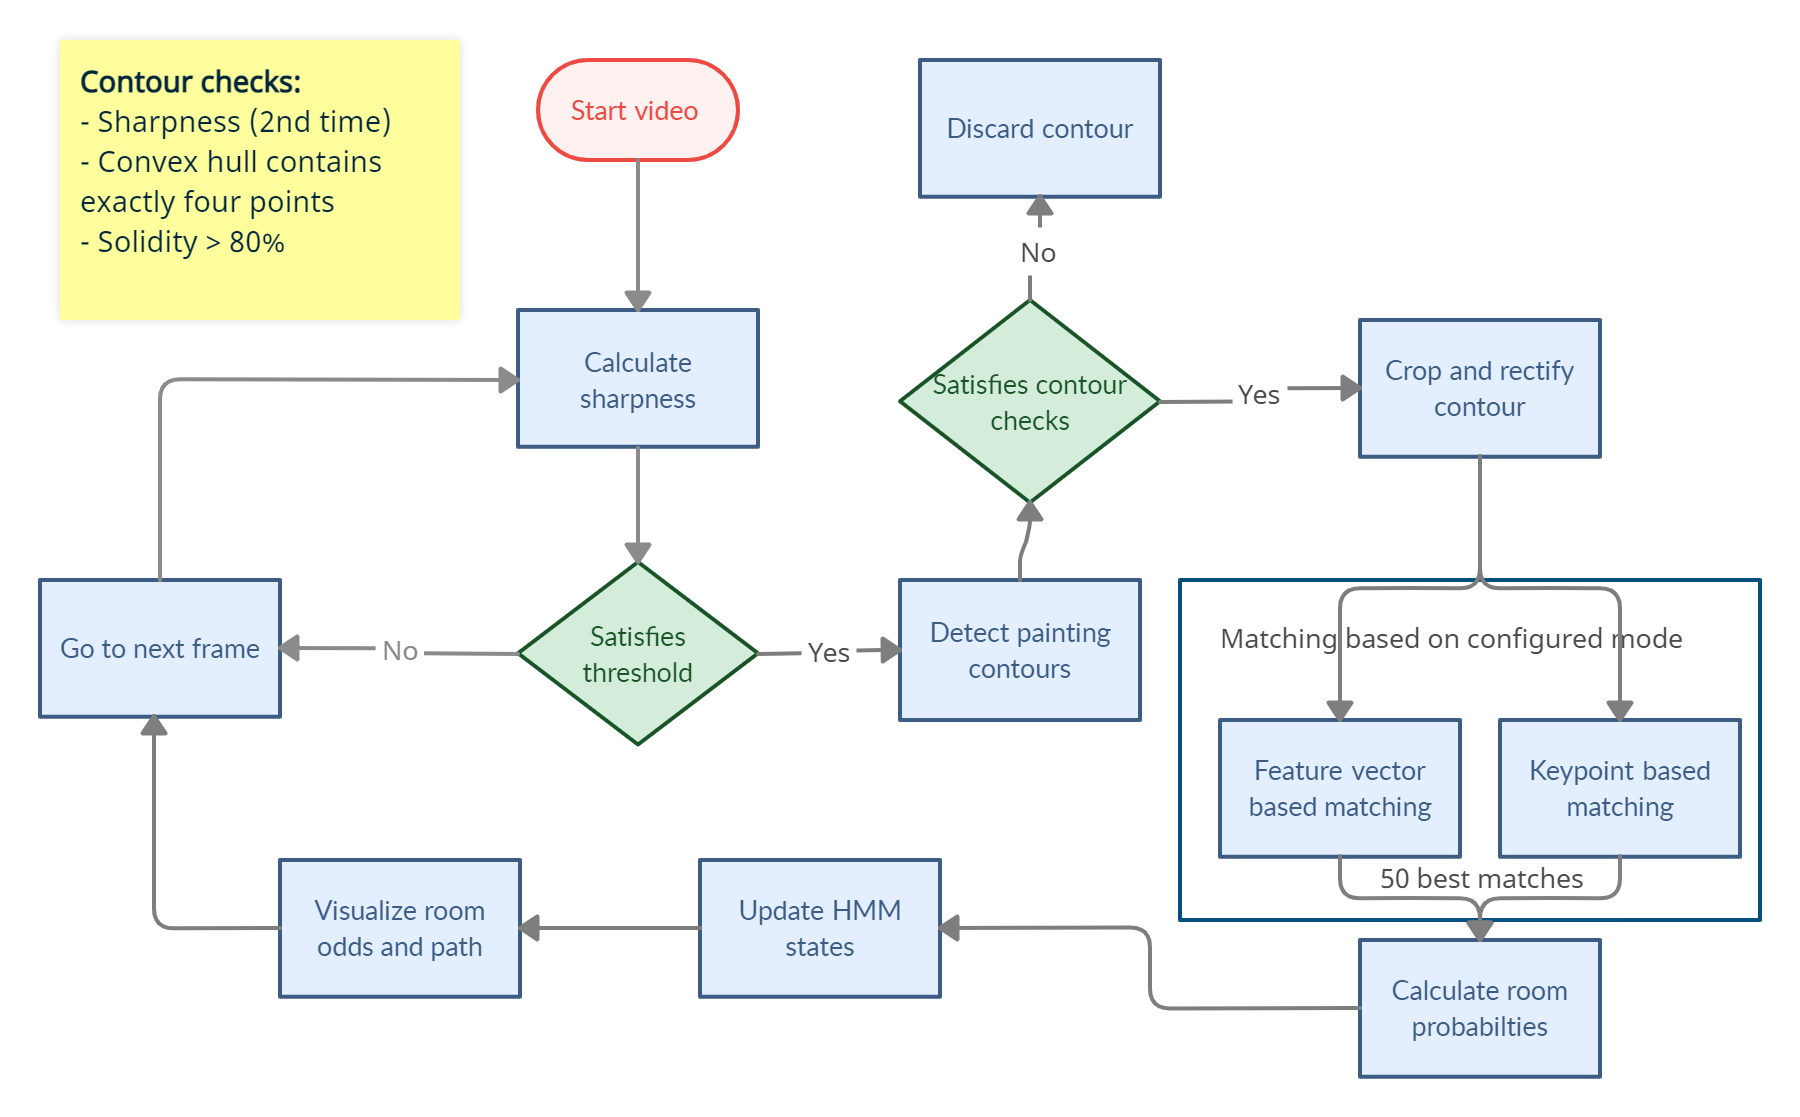
\includegraphics[width=\textwidth]{images/boxchart.png}
		\caption{Block diagram of the complete pipeline}
		\label{fig:blockdiagram}
	\end{minipage}%
\end{figure*}


% In feite wordt dit in het abstract beschreven
% Visual positioning prevents the necessity of a direct line of sight for signal transmissions or the scattering of beacons inside the building. When applied to the museum MSK Ghent it provides visitors with the number of the current room they are in. The visitors make videos of the route they take in the museum. From those videos, their location is determined. 


The final process is visualized in figure \ref{fig:blockdiagram}. The sequence of all steps ensures a working implementation.

First, the sharpness of the frame is calculated. When the sharpness is too low and doesn't satisfy the defined threshold, the frame is discarded. When the sharpness does satisfy the threshold, the frame is used to detect the painting contours. The detected painting contours are also checked. When the contours don't meet all the conditions, the frame is discarded. When the conditions are met, the painting is extracted, cropped, and rectified to get the frontal view.

After these steps, the matching itself starts. This is done with a combination of keypoint matching and feature vector matching. The best 50 matches from the database are sought. From those matches, the room probabilities (probabilities of the painting in a certain room) are calculated. The hidden Markov model then calculates the final room probabilities holding into account the location of the paintings in the previous frame. 

The predictions are then visualized with color on the floor plan of the MSK Ghent. Finally, the path most likely used by the user is also drawn on the floor plan.

When using the techniques on the videos, room for improvement can be determined (wrong matches, incorrect detections, etc.). Although remarkable good results are obtained. Next to improvements related to detection and wrong matching an optimization of the time each frame needs to compute may also be an improvement. This may be solved with multithreading. Nevertheless, the final implementation provides a good proof of concept considering various algorithms and techniques.


% In the final results, there are still some faults when running the program so there is of course still room for improvement. The program also requires a lot of processing powers. Nevertheless, it is a good working program. It can detect and match the painting's end determine the location of the user well. 


% \section{Results}

\bibliographystyle{IEEEtran}
\bibliography{references}
\end{document}
